\chapter{Projeto}


Este capítulo descreve o desenvolvimento prático do projeto, que é composto da detecção e \textit{tracking} de objetos dentro do software de referência, da utilização dos vetores calculados na estimativa de movimento para auxiliar no \textit{tracking} de objetos e da inserção dos metadados extraídos no bitstream. Primeiro são apresentados resultados práticos da inserção de mensagens \textit{SEI Userdata Unregistered} no bitstream de um vídeo codificado. Em seguida serão apresentados os novos módulos adicionados para realizar a extração e o armazenamento dos metadados e como eles foram integrados ao software de referência. Por fim será apresentada uma avaliação dos resultados obtidos.


\section{Inserindo userdata no Bitstream}


O H.264 possui uma sintaxe específica para o envio de mensagens não necessárias ao processo de decodificação, embutidas no bitstream de vídeo, são mensagens SEI (\textit{Supplemental Enhanced Information}). Ao longo dessa seção será estudada a utilização prática das mensagens SEI do tipo \textit{UserData} não registrada em pontos diferentes no processo de codificação. 


\subsection{Ambiente de teste}

Todos os testes foram realizados com o mesmo trecho de vídeo obtido a partir do site http://media.xiph.org/video/derf.

O vídeo possui a seguinte configuração:

\begin{itemize}
        \item quadros por segundo = 29.97.
        \item total de quadros    = 300.
        \item comprimento         = 176 pixels.
        \item altura              = 144 pixels.
        \item espaço de cor       = YUV, 4:2:0.
\end{itemize}

Para testar a conformidade do bitstream gerado foi utilizado o decodificador de referência, após utilizar o decodificador de referência para transformar o bitstream H.264 em vídeo raw foi utilizado o Gstreamer para exibir o vídeo e constatar visualmente que o vídeo foi decodificado sem problemas.

O bitstream também foi testado diretamente no Gstreamer, pra verificar se o bitstream tocaria em um player usual (muitos players open source utilizam gstreamer como framework de multimedia). 

Gstreamer utiliza internamente o ffmpeg para fazer o decoding do bitstream H.264. 


\subsection{Enviando uma mensagem SEI Userdata}

Inicialmente foi utilizada a opção \textit{GenerateSEIMessage} do próprio codificador, onde é possível ativar o envio de uma mensagem e configurar a mensagem que será enviada. Mas isso serve apenas para testes bem simples já que apenas uma mensagem é enviada ao longo de todo o bitstream de vídeo, e em forma de texto. Essa função é invocada no módulo \textit{filehandle}, por isso ele foi escolhido como ponto de partida para testes de inserção de mensagens SEI no bitstream.

A partir do que foi observado na presente implementação de envio de mensagens SEI não registradas foi desenvolvida uma nova função que consegue criar uma mensagem SEI com qualquer tipo de dado, não sendo necessariamente texto. Para testar essa nova função foram feitas pequenas alterações no módulo filehandle do codificador, na função \textit{start\_sequence}, e foi adicionado um novo módulo \textit{udata\_gen} para possibilitar a criação de mensagens SEI a partir de um char* e do seu tamanho.

Também foram realizadas alterações no decodificador para realizar a extração da mensagem SEI, para isso foi criado um novo módulo \textit{udata\_parser} que faz a extração dos dados a partir de um SEI NALU que possui uma mensagem SEI do tipo \textit{UserData} não registrada.

O módulo \textit{udata\_parser} é chamado dentro do módulo sei (\textit{sei.c}) do decodificador (\textit{ldecod}), na função \textit{InterpretSEIMessage} que trata a recepção de mensagens SEI. Nesse ponto as informações são enviadas para o \textit{stdout}, para constatar se as mensagens foram extraídas corretamente.

Com essas duas alterações prontas foi possível testar o envio de um \textit{SEI User Data} não registrado contendo informação que não é necessariamente texto (nesse caso a ideia é que fossem parâmetros extraídos do video). 

Foi constatado que:

\begin{itemize}
        \item As informações persistiram no bitstream e foram extraídas com sucesso pelo decodificador de referência modificado.
        \item O decodifica de referência realizou a decodificação do vídeo com sucesso, gerando um arquivo de vídeo bruto válido com todo o vídeo original.
        \item O bitstream H.264 gerado mostrou ser compatível com Gstreamer.
\end{itemize}

Portanto não seria um problema enviar dados de qualquer natureza utilizando mensagens \textit{SEI User Data} não registradas, o decodificador de referência continuou funcionando sem problemas e a mensagem permaneceu íntegra. Até mesmo um decodificador de terceiro (ffmpeg + Gstreamer) funcionou com o bitstream gerado.


\subsection{Enviando diversas mensagens SEI Userdata de tamanho variado}


Após ter enviado uma mensagem com sucesso o próximo passo foi enviar várias mensagens no mesmo bitstream, com tamanhos variados. Porém surgiram dois problemas, a quantidade de mensagens \textit{SEI Userdata} que podem ser enviadas no mesmo bitstream e o tamanho máximo delas. De acordo com \cite{ituh264avc} não existe um limite explicito nem na quantidade, nem no tamanho das mensagens SEI.

Porém na prática, além dos limites implícitos que podem existir por causa do nível de conformidade do codificador, muitos decodificadores possuem limites no que eles suportam que estão relacionados com a maneira como eles foram implementados e não com a recomendação em si. 

Alguns decodificadores possuem limites de quantas mensagens SEI podem receber, outros simplesmente descartam mensagens SEI. Como a variedade de decodificadores é muito grande, o foco da implementação será o codificador/decodificador de referência.

No codificador de referência existe um limite explicito no tamanho máximo de um NALU, esse limite é definido no arquivo \textit{lcommon/inc/nalucommon.h} como \textit{MAXNALUSIZE}. O valor desse limite é 64000 bytes. Ao longo dos testes esse será o tamanho máximo utilizado.

Para testar o envio de múltiplos SEI NALUS com mensagens \textit{SEI Userdata} de tamanhos variados, respeitando o limite de 64000 bytes, foi criada uma nova função no módulo \textit{udata\_gen} que gera uma \textit{string} maior a cada nova chamada. 

Ao atingir o tamanho limite a função retorna ao tamanho inicial e reinicia o processo de aumento da string. Dessa maneira é possível enviar diversas mensagens todas de tamanho diferente, explorando desde mensagens de tamanho pequeno como de mensagens que cheguem perto do tamanho máximo.

Foi feita uma alteração no módulo \textit{filehandle} do codificador, para criar e escrever no bitstream 1000 mensagens de tamanho variado. Nenhuma alteração foi necessária no decodificador.

Foi constatado que:

\begin{itemize}
        \item Os 1000 SEI NALUs persistiram no bitstream e foram extraídos com sucesso pelo decodificador de referência modificado.
        \item O decodifica de referência realizou a decodificação do vídeo com sucesso, gerando um arquivo de vídeo bruto válido com todo o vídeo original.
        \item O bitstream H.264 gerado com os 1000 SEI NALUS mostrou ser compatível com Gstreamer.
\end{itemize}

Portanto não seria um problema enviar múltiplos SEI NALUs no mesmo bitstream, e de tamanho variado, desde que se respeite o tamanho máximo definido pelo software de referência. A única limitação deste teste é que os SEI NALUs são escritos no bitstream sequencialmente, não estão intercalados com os NALUs de vídeo e são todos escritos no inicio do bitstream, antes dos quadros de vídeo.

Foi realizado um teste para constatar se múltiplos SEI NALUs vão funcionar bem intercalados com quadros de vídeo. Para isso foram utilizadas as mesmas funções já existentes nos testes anteriores, mas ao invés de os SEI NALUs serem inseridos no módulo \textit{filehandle} eles são inseridos no módulo \textit{lencod}, após a geração de cada quadro. 

Como o vídeo consiste em 300 quadros, foram inseridos exatamente 300 SEI NALUs, sempre que um quadro é escrito no bitstream um SEI NALU de tamanho variável é escrito após ele.

Foi constatado que:

\begin{itemize}
        \item Os 300 SEI NALUs persistiram no bitstream e foram extraídos com sucesso pelo decodificador de referência modificado.
        \item O decodificador de referência realizou a decodificação do vídeo com sucesso, gerando um arquivo de vídeo bruto válido com todo o vídeo original.
        \item O bitstream H.264 gerado com os 300 SEI NALUS mostrou ser compatível com Gstreamer.
\end{itemize}

Utilizando mensagens \textit{SEI Userdata} não registradas é possível enviar dados que não fazem parte do processo de decodificação, de tamanhos variados (respeitando o tamanho máximo estipulado pelo software de referência), em posições variadas dentro do bitstream e em quantidades variadas. O código fonte de todos os módulos alterados no software de referência e dos novos módulos, que foram utilizados para realizar esse teste, se encontra no apêndice A.


\section{ Módulo extracted\_metadata }


Esta seção explica detalhadamente a implementação do módulo \textit{extracted\_metadata}. Ele é escrito em linguagem C e foi adicionado no diretório \textit{lcommon} do software de referência já que ele é utilizado tanto pelo codificador como pelo decodificador. Todas as funções são declaradas no cabeçalho \textit{lcommon/inc/extracted\_metadata.h} e implementadas em \textit{lcommon/src/extracted\_metadata.c}.

Apesar de ser escrito em C, foi utilizada uma abordagem orientada a objetos. A orientação a objetos é feita internamente de uma maneira bem simples, a classe pai possui uma lista de ponteiros de função e na construção da classe filho ela fornece a implementação para essas funções.

A classe pai pode realizar alguma atividade antes ou depois da chamada da função implementada pela classe filho. Dessa maneira fica fácil a classe pai executar código que é comum a todas as subclasses, antes de chamar a função implementada pela subclasse. Isso foi especialmente útil na implementação da serialização, cada implementação de metadado deve se preocupar apenas com a serialização dos seus dados, sem se preocupar com os dados da classe pai, já que a classe pai irá serializar esses dados antes de chamar a função de serialização da classe filho, simplificando a implementação de novos metadados.

Funções da família \textit{hton}, definidas em \textit{arpa/inet.h}, foram utilizadas na serialização dos metadados para garantir que ao serializar os dados os bytes estejam de acordo com o padrão para rede. Na desserialização, funções da família \textit{ntoh} foram utilizadas para garantir que os bytes ordenados de acordo com o padrão para rede fossem convertidos para a ordenação de \textit{bytes} do \textit{host}.

O padrão utilizado nos nomes das funções é \textit{nome\_do\_tipo\_método}. Por exemplo a implementação em C do método \textit{new} da classe ExtractedMetadataBuffer será \textit{extracted\_metadata\_buffer\_new}. Por classe entende-se a estrutura definida com o determinado nome, e sempre ao chamar uma função que é método desta classe, o primeiro parâmetro é um ponteiro para a estrutura que representa a classe. Ao longo dessa seção será feita referência apenas ao nome dos métodos, e não ao nome completo da função que está implementada em C.

Na figura ~\ref{fig:extracted_metadata_class_diagram} pode ser visto o diagrama de classe dos objetos definidos no módulo. A descrição de cada um dos objetos são apresentados nessa seção. 


\begin{figure}[H]
\centering
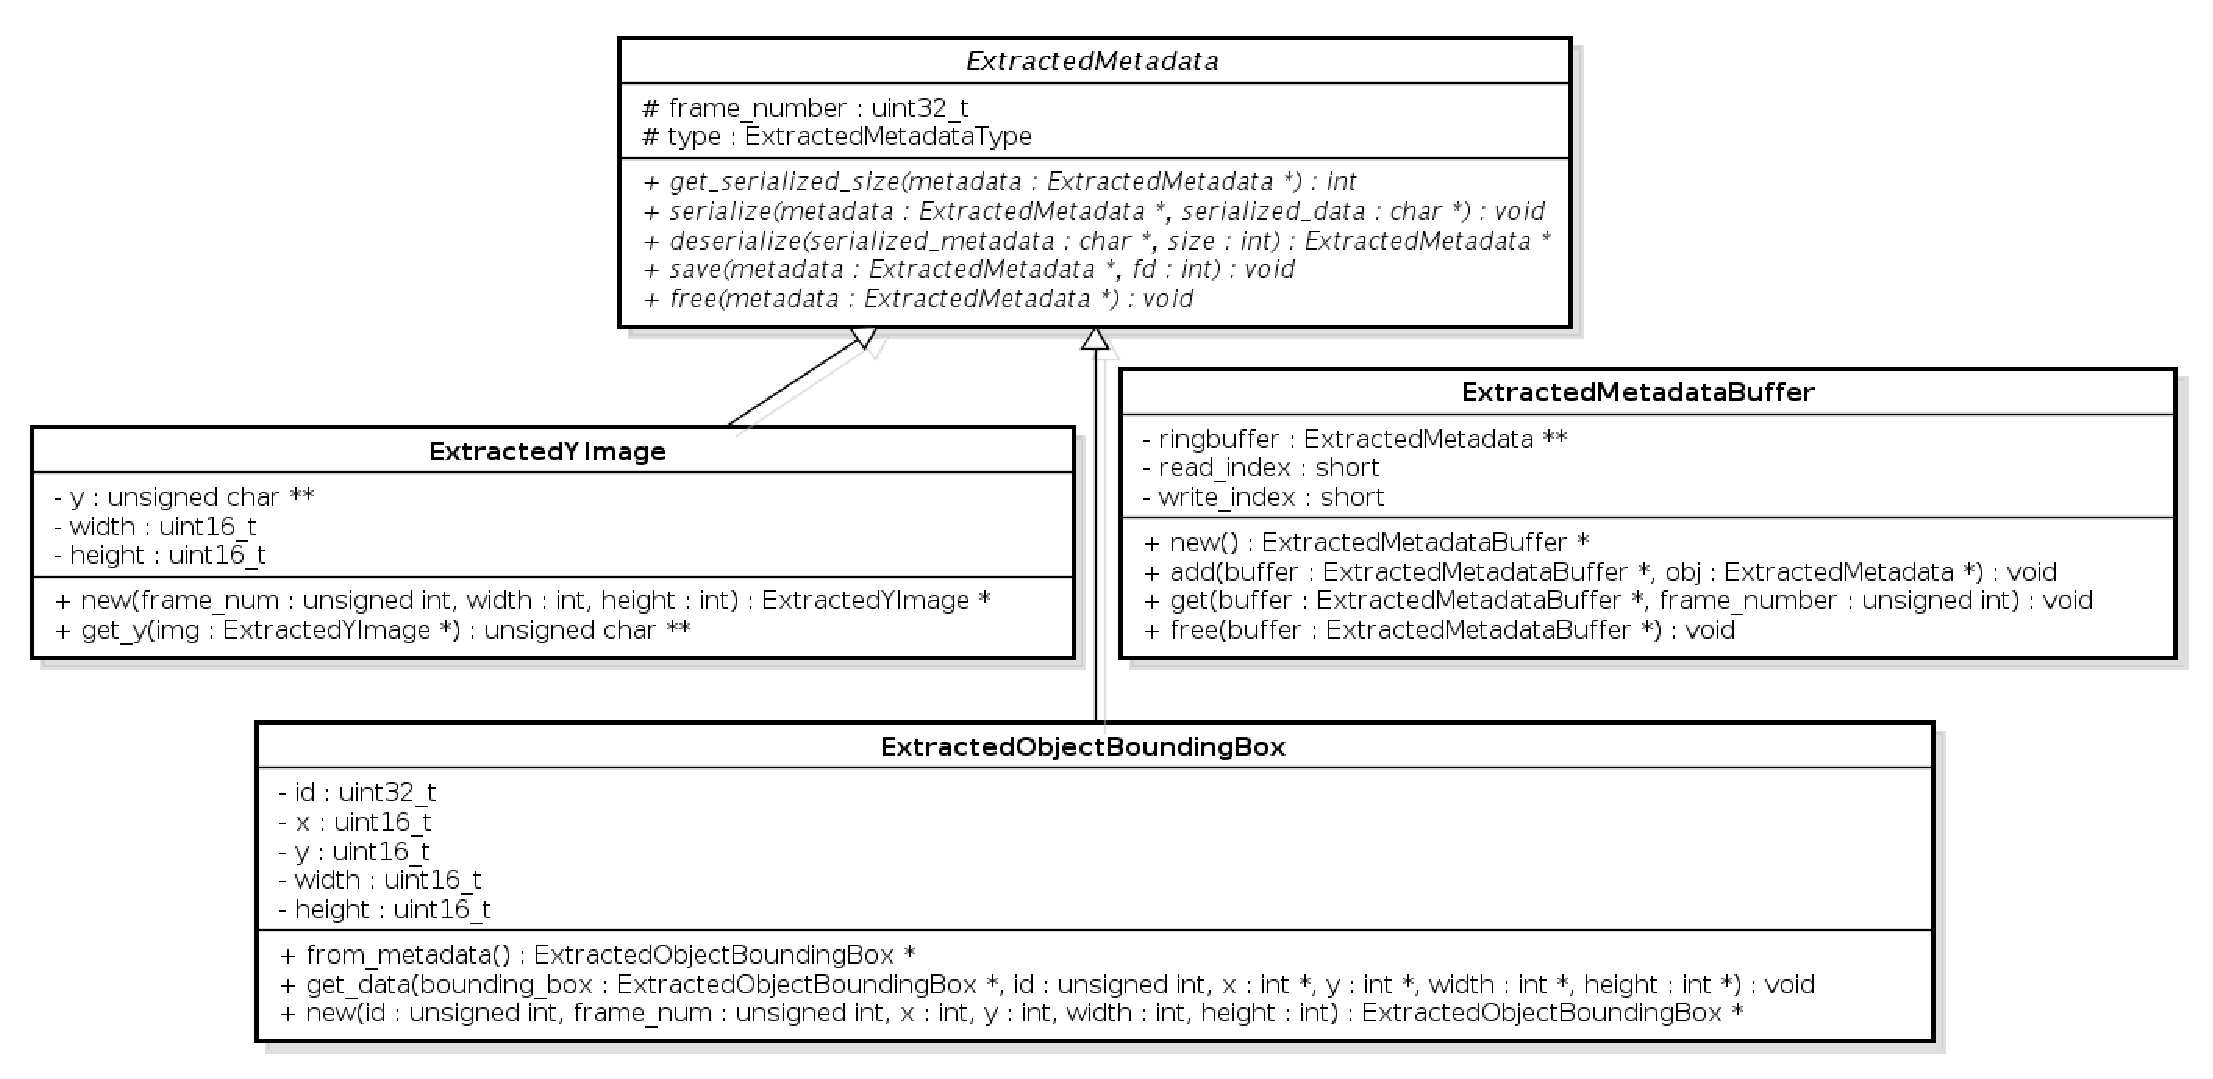
\includegraphics[scale=0.45]{imagens/fig10.eps}
\caption{Diagrama de classe dos objetos definidos no módulo extracted\_metadata.}
\label{fig:extracted_metadata_class_diagram}
\end{figure}

A implementação deste módulo encontra-se no apêndice B.


\subsection{ Extracted\_Metadata }

Esta classe abstrai a serialização, desserialização, salvamento e destruição dos diferentes tipos de metadados. O método \textit{serialize} é responsável pela serialização, que  é utilizada na inserção de um metadado no bitstream (utilizado em conjunto com o módulo \textit{udata\_gen}). 

O método \textit{get\_serialized\_size} é utilizado para auxiliar a alocação de memória necessária pelo processo de serialização, dessa maneira fica a cargo de quem está serializando o metadado alocar a memória necessária para a serialização e liberar a memória após o uso.

\begin{figure}[H]
\centering
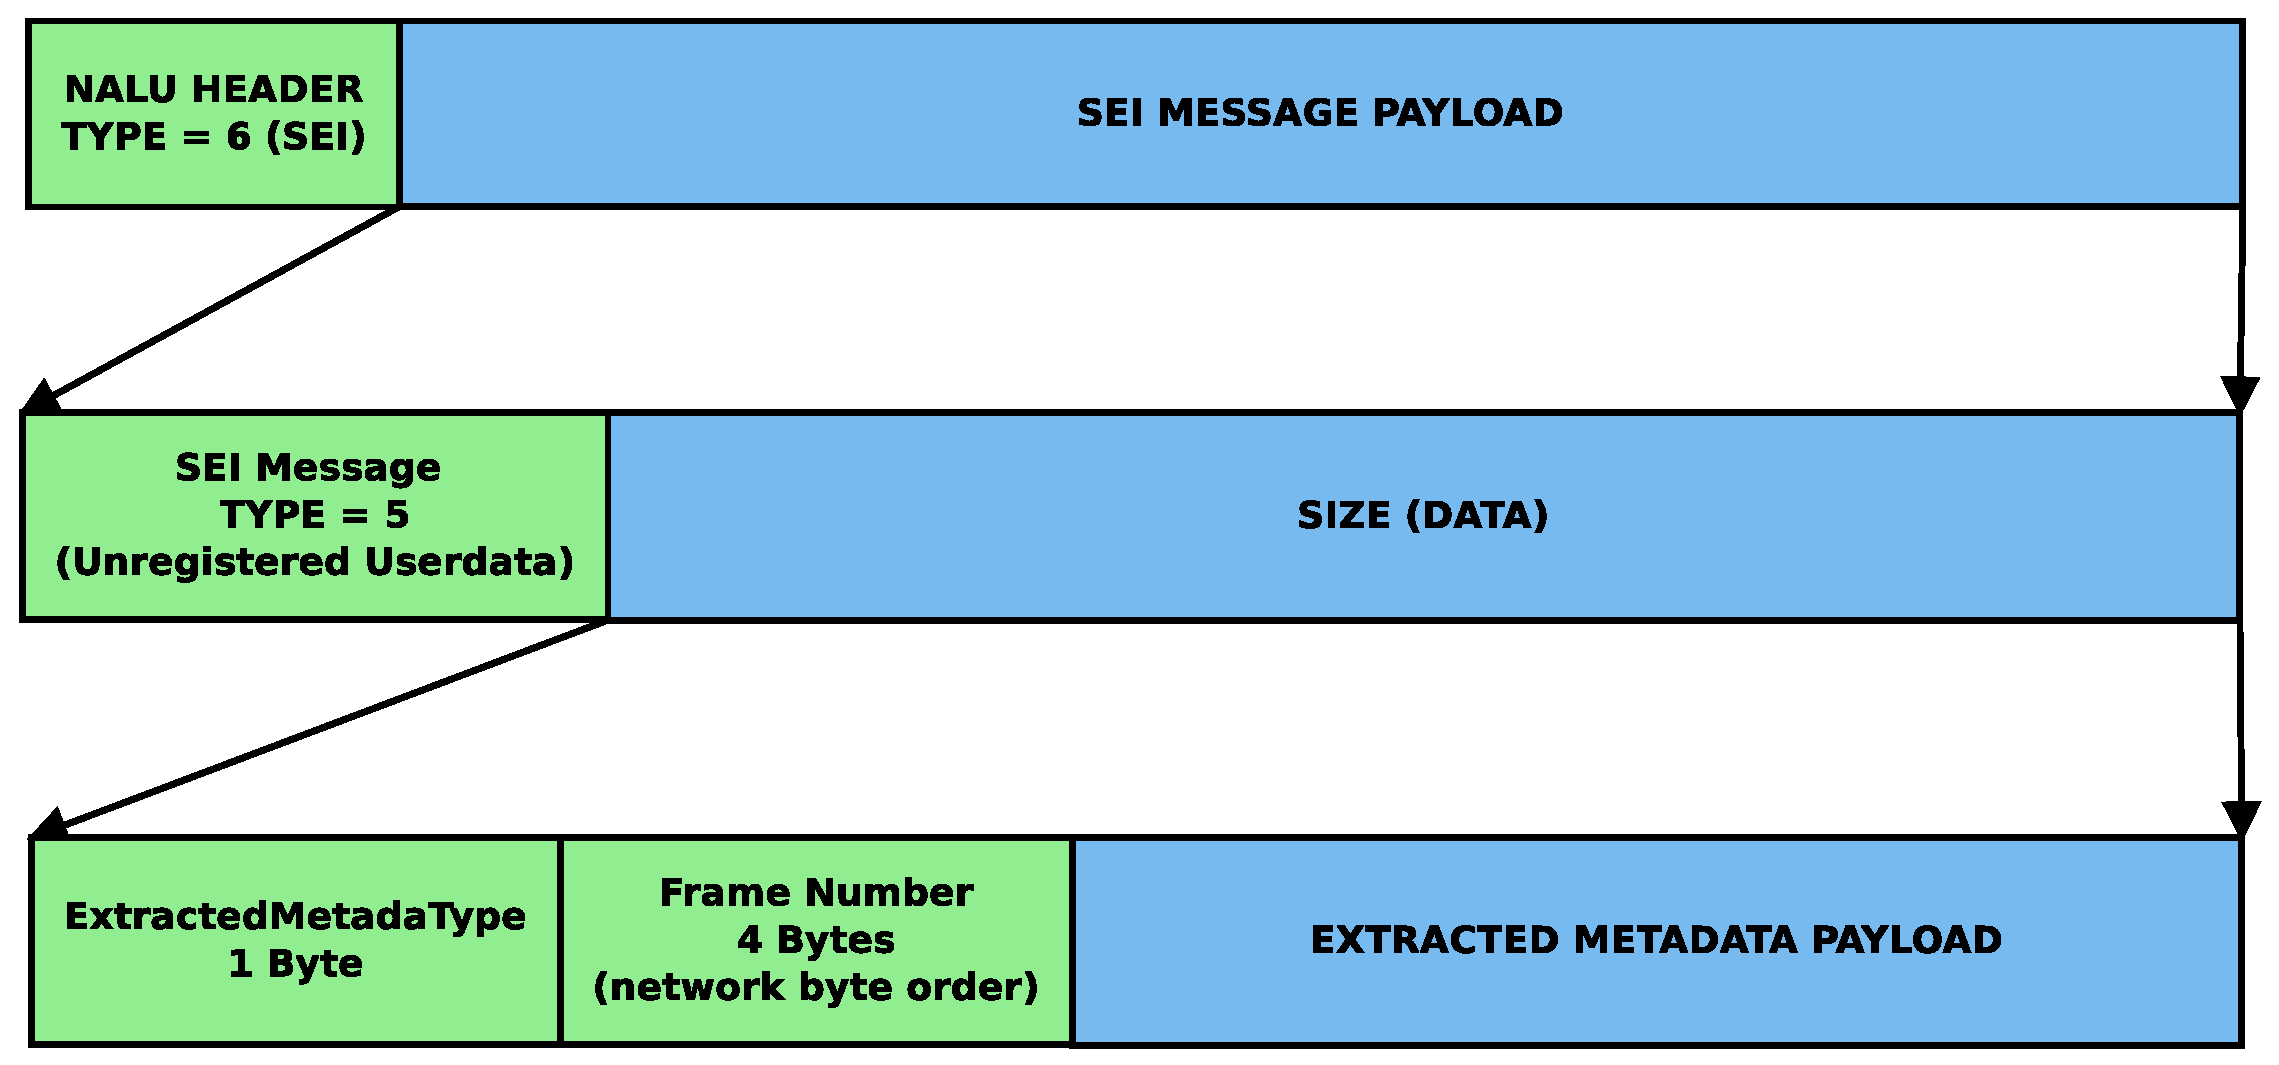
\includegraphics[scale=0.4]{imagens/fig9.eps}
\caption{Metadado serializado dentro de um NALU do tipo SEI. Cabeçalho em verde, \textit{payload} em azul.}
\label{fig:extracted_metadata_on_nalu}
\end{figure}

Como pode ser visto na figura ~\ref{fig:extracted_metadata_on_nalu}, um metadado serializado sempre começa com o seu tipo e o número do quadro (em ordem de apresentação) do qual ele foi extraído. O payload do metadado será definido pela classe que herdar \textit{ExtractedMetadata}.

O método \textit{save} salva o metadado em um file descriptor, sendo útil para realizar depuração. O método \textit{free} libera todos os recursos utilizados pelo metadado.


\subsection{ Extracted\_Y\_Image }


Esta classe herda \textit{ExtractedMetadata} e representa o plano luma de um objeto de interesse, é composto basicamente do plano luma com o seu comprimento e altura. O plano luma é um \textit{array} bidimensional de bytes, onde cada byte é o valor de um pixel. A primeira dimensão do array é a linha (Y) que vai de 0 á altura - 1. A segunda dimensão é a coluna (X), que vai de 0 á comprimento - 1.

Ao detectar um objeto de interesse é possível extrair apenas o objeto e inserir ele no bitstream. O objeto pode ser recuperado no decodificador e salvo em um arquivo. Como ele é composto apenas do plano luma só é possível visualizar o objeto monocromático. Muitos algoritmos trabalham com imagens monocromáticas, esse metadado pode ser utilizado para preservar no bitstream o objeto original antes que parte das informações dele possam ser destruídas pelo processo de codificação, dependendo do nível de perda do processo da codificação. 

Em alguns casos para economizar largura de banda na transmissão, ou espaço no armazenamento, o vídeo é obtido em alta definição mas tem seu tamanho reduzido, utilizando esse metadado seria possível dispor de um banco de objetos de interesse em alta resolução apesar dos vídeos terem seu tamanho reduzido.

Para criar um objeto \textit{ExtractedYImage} basta utilizar o método \textit{new} passando como parâmetro o número do quadro, seu comprimento e sua altura. Pela altura e comprimento informados será alocado o plano, que pode ser obtido através do método \textit{get\_y}, tendo obtido o plano basta escrever nele o plano luma do objeto e o metadado estará pronto para ser serializado e inserido no bitstream.


\begin{figure}[H]
\centering
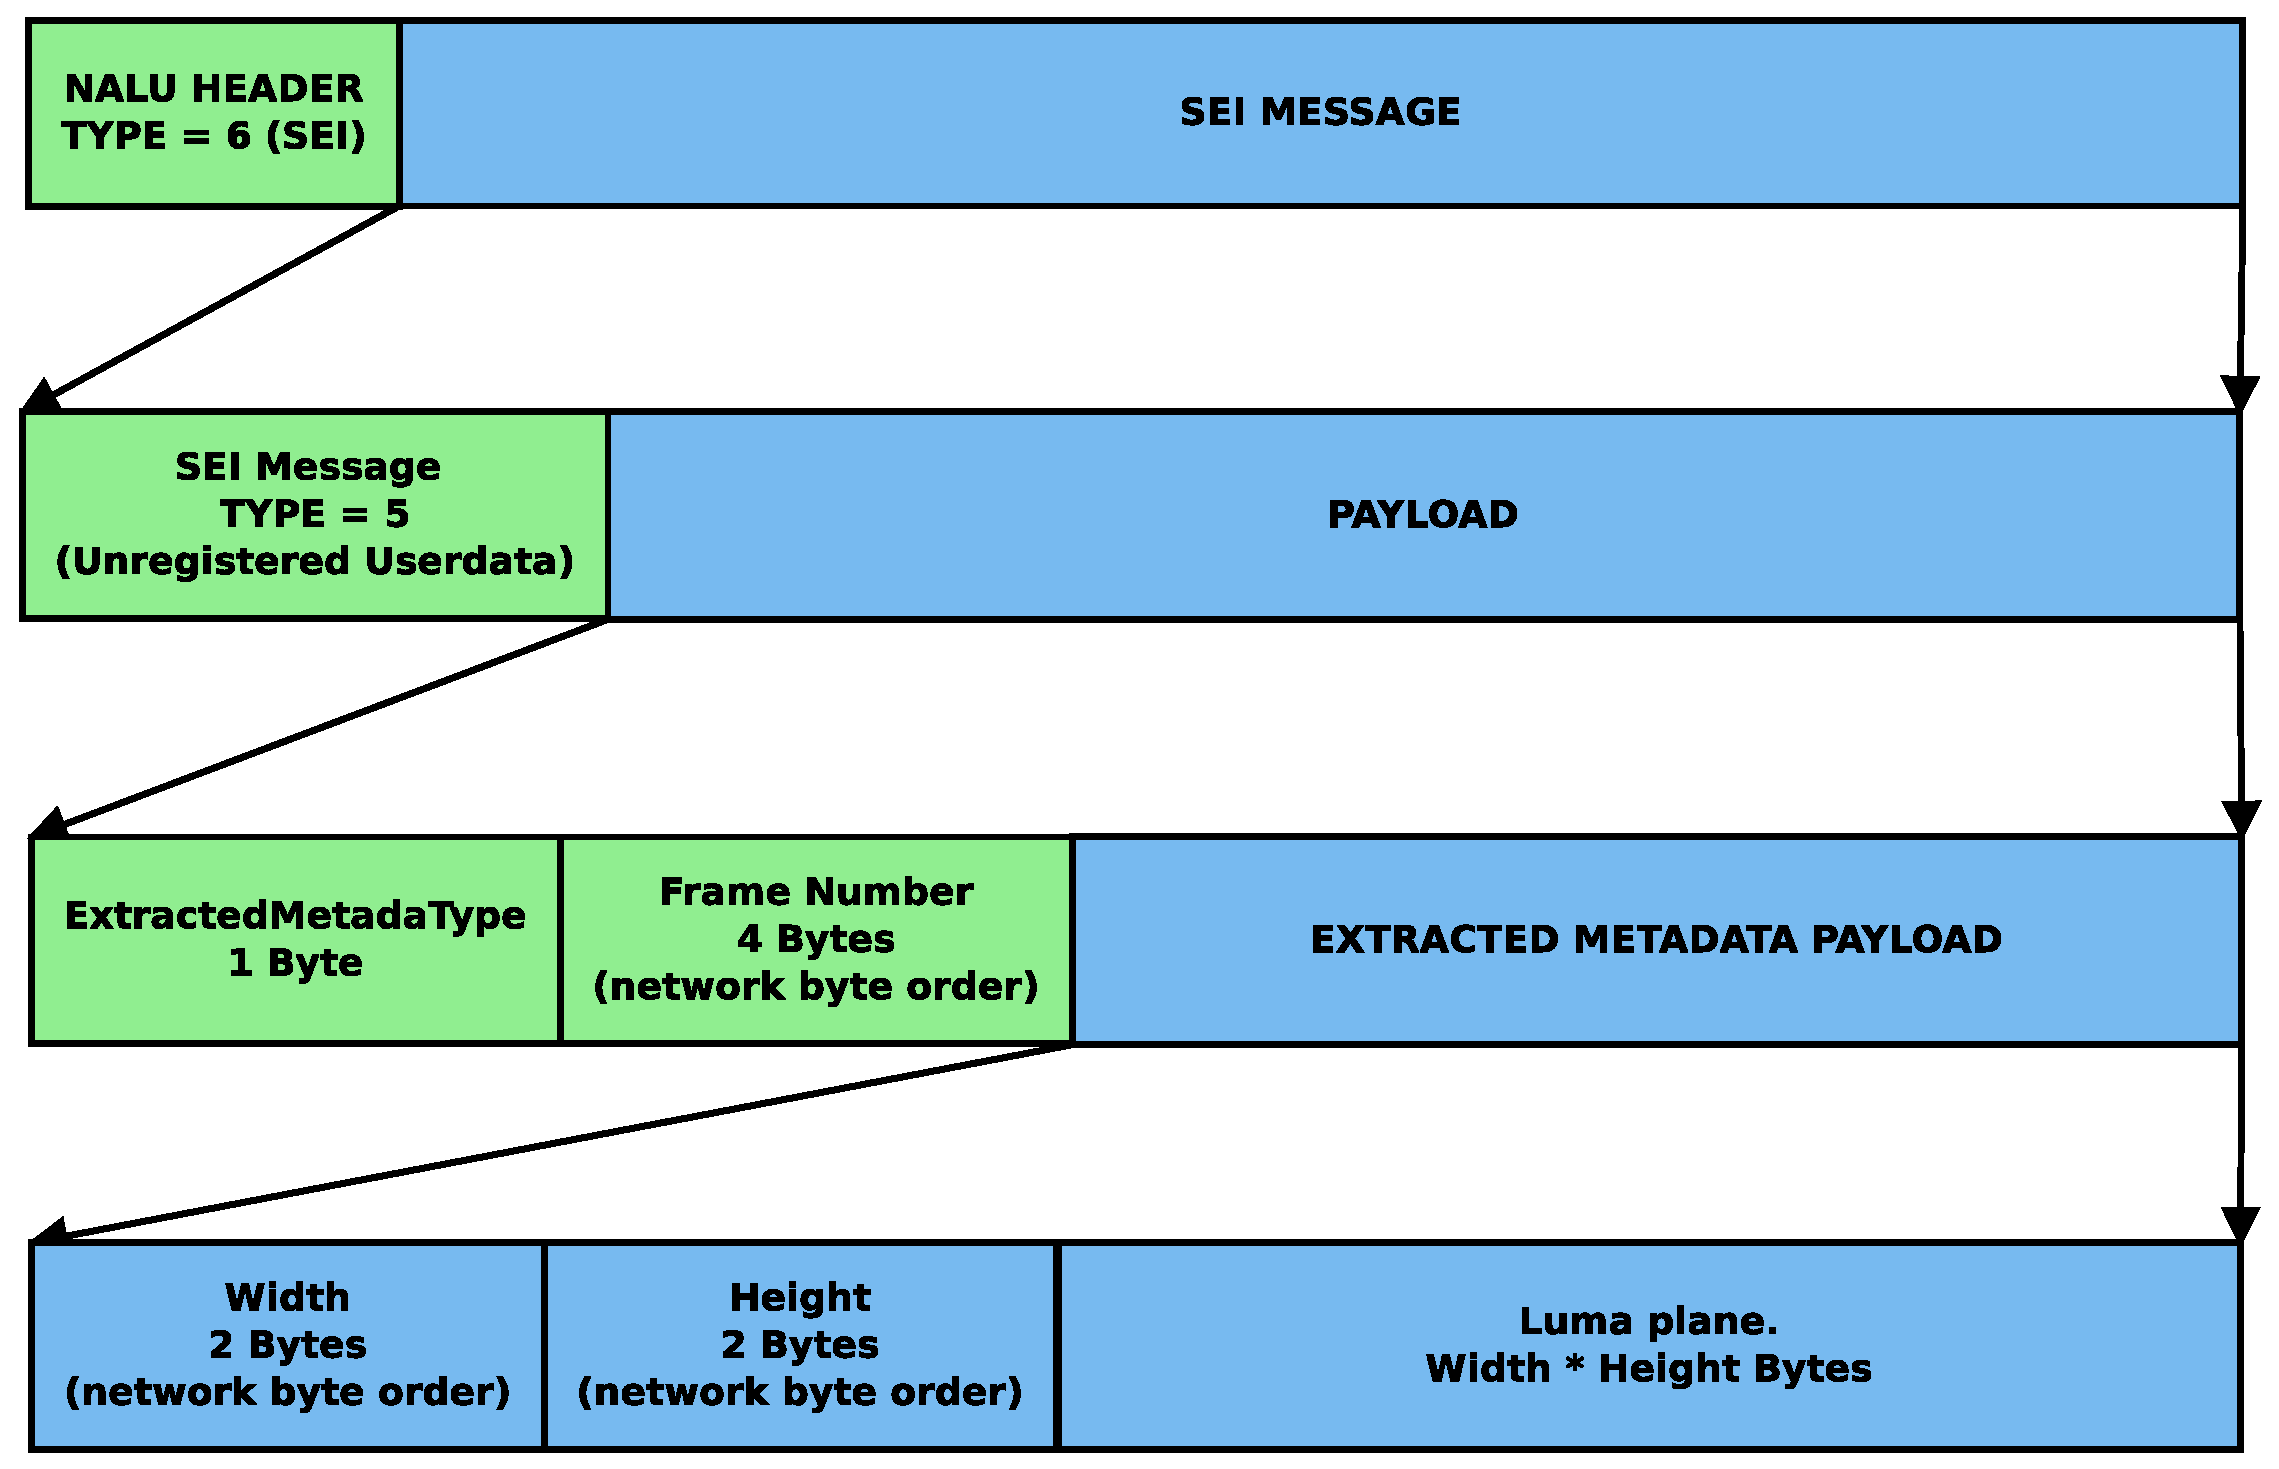
\includegraphics[scale=0.4]{imagens/fig11.eps}
\caption{Objeto ExtractedYImage serializado dentro de um NALU do tipo SEI. Cabeçalho em verde, \textit{payload} em azul.}
\label{fig:extracted_y_image_on_nalu}
\end{figure}


\subsection{ Extracted\_Object\_Bounding\_Box }


Esta classe herda \textit{ExtractedMetadata} e representa uma caixa delimitadora envolta de um objeto de interesse. Ela é composta de um identificador único do objeto, as coordenadas (x, y) da caixa, sua altura e seu comprimento.

Ao ocorrer a detecção de um objeto de interesse é possível inserir no bitstream um metadado \textit{ExtractedObjectBoundingBox}, ao ser recuperado no decodificador, utilizando o identificador único, é possível realizar a indexação de todos os objetos diferentes detectados ao longo do vídeo. Como a classe pai \textit{ExtractedMetadata} possui o número do quadro em ordem de apresentação, é possível dizer em que momento do vídeo o objeto foi detectado pela primeira vez e qual o momento que ele foi identificado pela última vez, tendo assim todo o intervalo de tempo em que o objeto esteve no vídeo.

Com as informações da caixa delimitadora também é possível desenhar a caixa diretamente no vídeo, facilitando a constatação visual de que um objeto de interesse está presente no trecho de vídeo. Se para cada quadro que possui o objeto de interesse for inserido um metadado \textit{ExtractedObjectBoundingBox} no bitstream será possível realizar o tracking do objeto ao longo do vídeo. 

Para criar um objeto \textit{ExtractedObjectBoundingBox} basta utilizar o método \textit{new} passando como parâmetro o identificador do objeto, o número do quadro (em ordem de apresentação), a coordenada x, a coordenada y, seu comprimento e sua altura. Após a construção basta serializar e inserir o objeto \textit{ExtractedObjectBoundingBox} no bitstream. 

Ao recuperar o metadado do bitstream o método \textit{get\_data} pode ser utilizado para se obter informações como o identificador único do objeto, suas coordenadas e seu tamanho.


\begin{figure}[H]
\centering
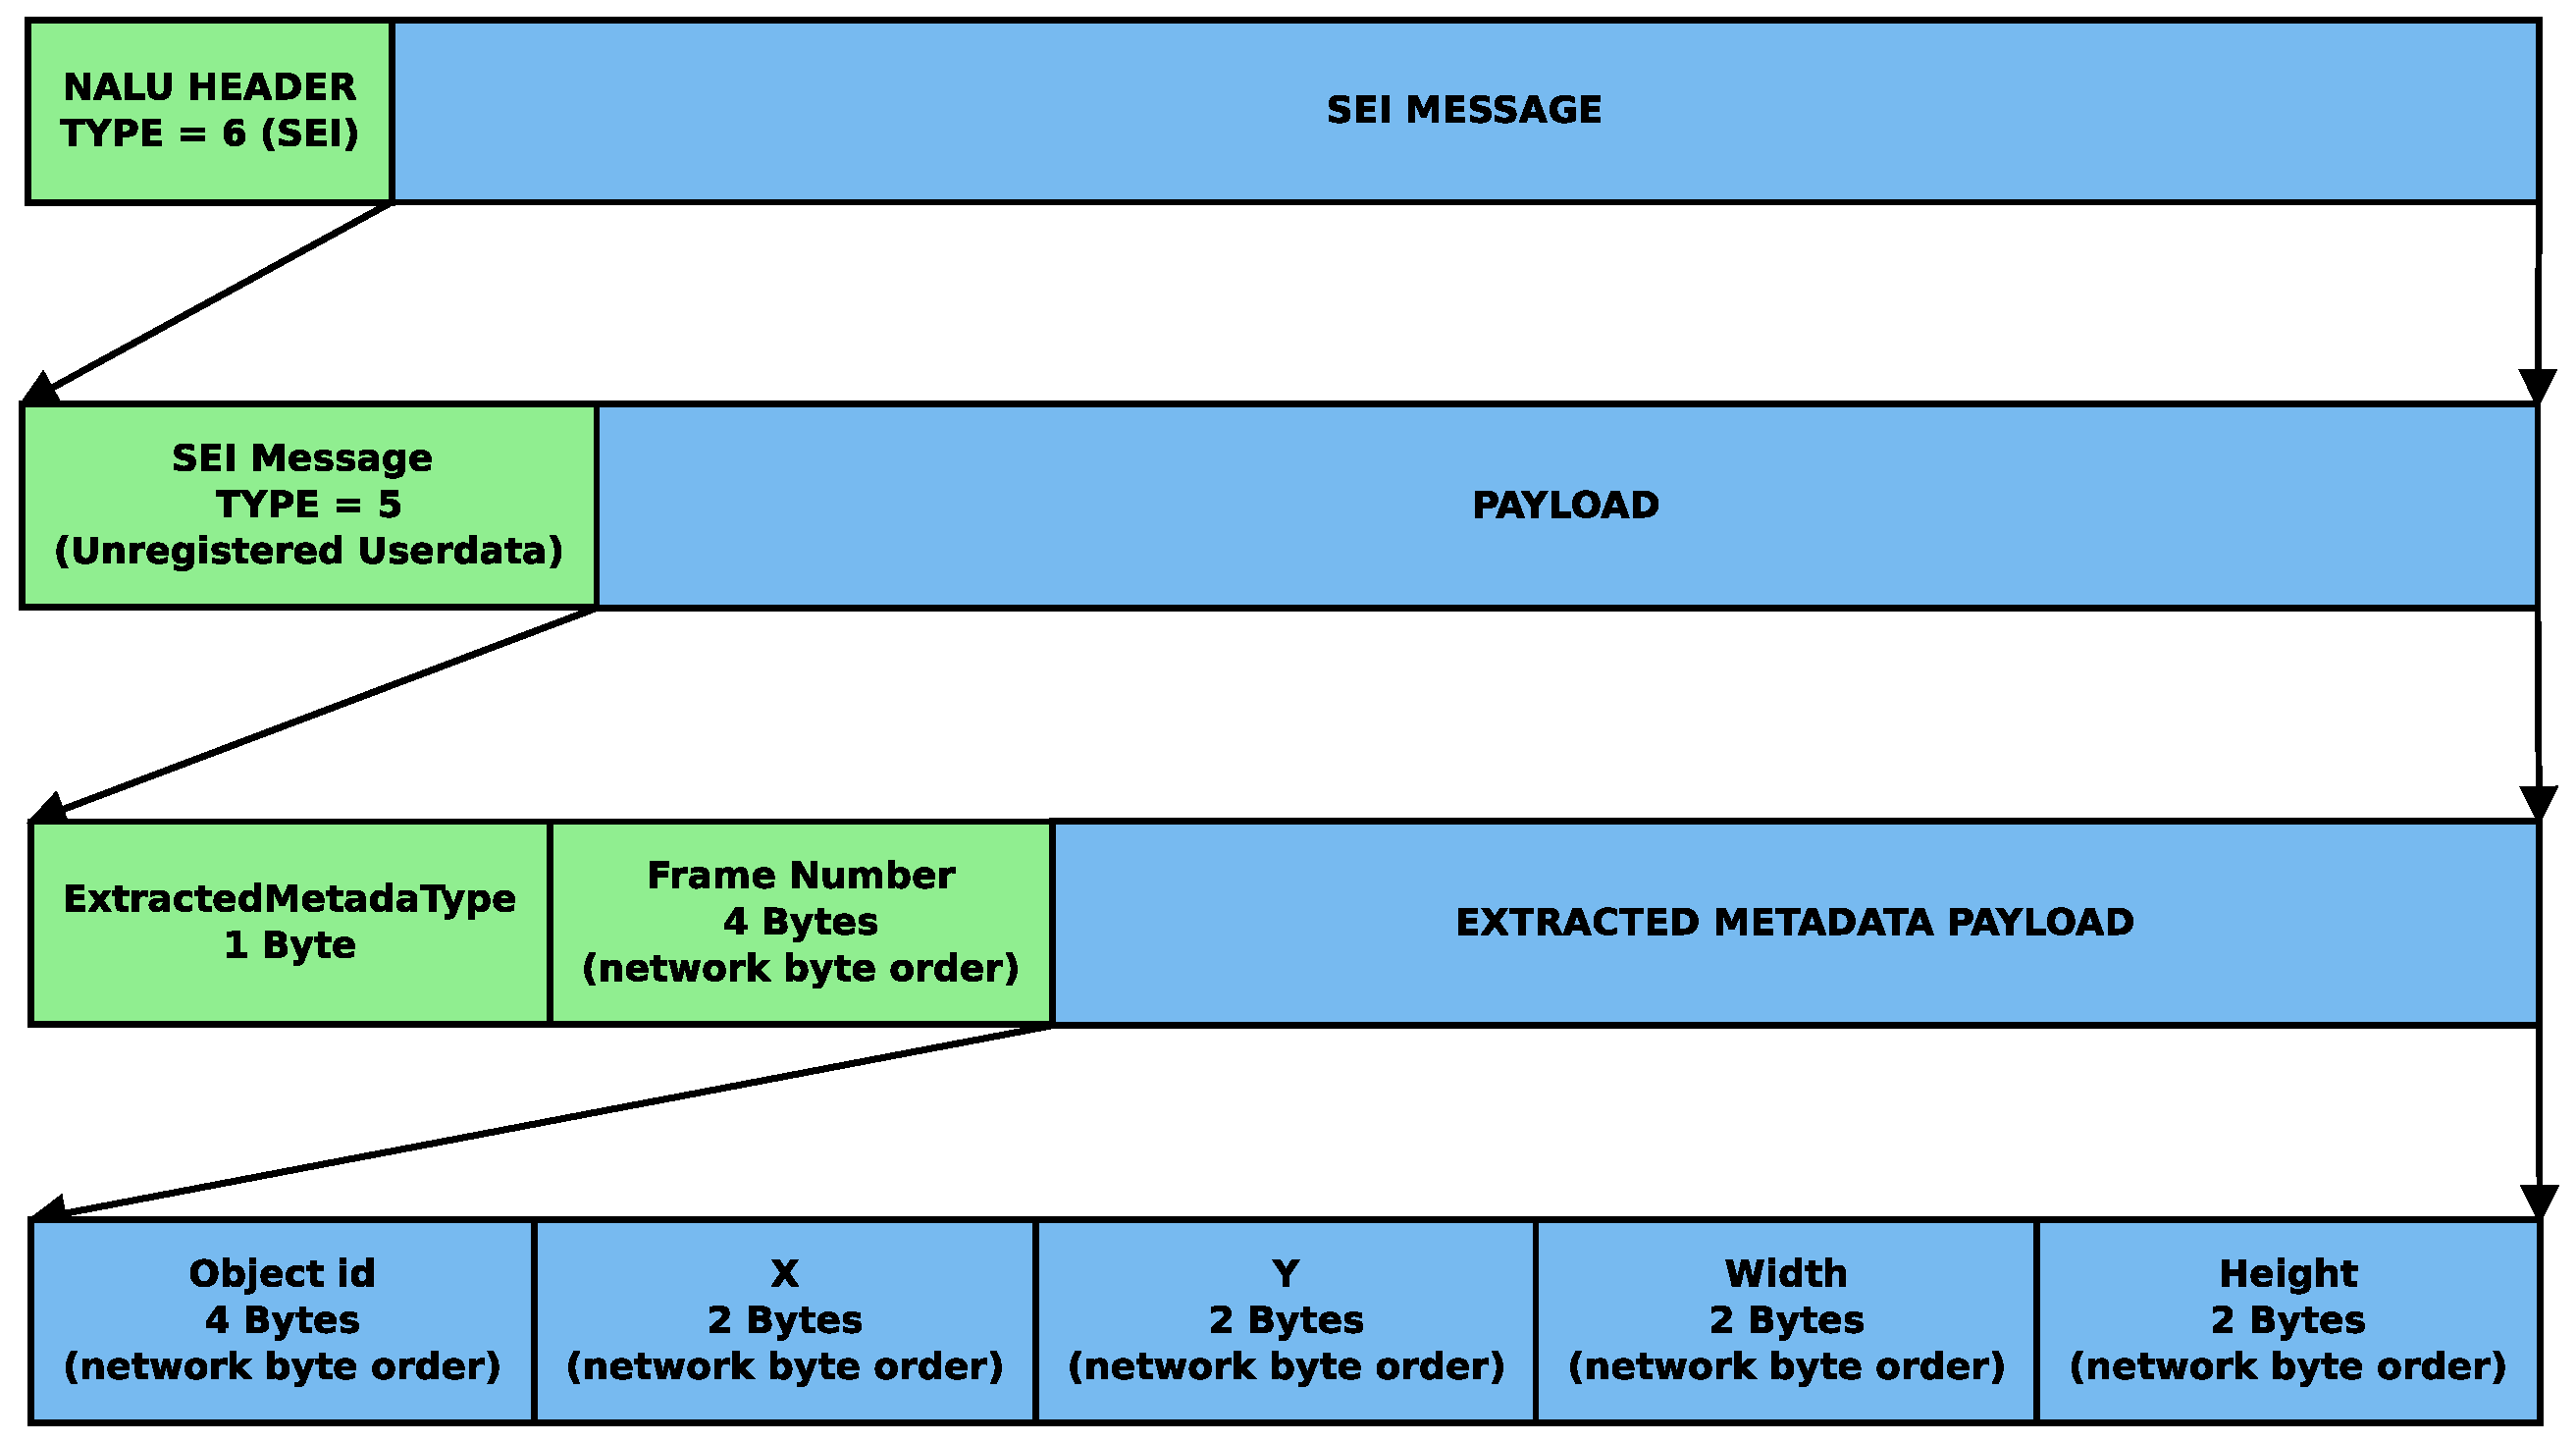
\includegraphics[scale=0.4]{imagens/fig12.eps}
\caption{Objeto ExtractedObjectBoundingBox serializado dentro de um NALU do tipo SEI. Cabeçalho em verde, \textit{payload} em azul.}
\label{fig:extracted_object_bounding_box_on_nalu}
\end{figure}


\subsection{ Extracted\_Metadata\_Buffer }

Esta classe é utilizada para bufferizar diversos metadados extraídos no processo de decodificação. O método \textit{add} adiciona um novo metadado no buffer, os metadados podem ser recuperados do buffer utilizando o método \textit{get}, neste método deve ser informado o número do quadro em ordem de apresentação, se houver algum metadado referente a este quadro ele será retornado, se não existir o método retornará \textit{NULL}.

O buffer foi construído porque nem sempre os metadados ficam no bitstream exatamente antes do quadro ao qual eles pertencem. Dependendo do vídeo vários metadados podem ser inseridos no bitstream antes que um quadro seja escrito no bitstream, dessa maneira é necessário bufferizar os metadados no decodificador até terminar a decodificação de um quadro e chegar o momento de apresentá-lo. Ao terminar a decodificação o buffer pode ser consultado para verificar se existe algum metadado referente ao quadro que será apresentado.

Para tornar a bufferização eficiente e simples não existe nenhum tipo de ordenação dos metadados dentro do buffer, ao se obter o metadado para um determinado quadro, qualquer metadado que for referente a um quadro anterior será descartado pelo buffer. Portanto um metadado deve ser gravado no bitstream antes do quadro do qual ele foi extraído. E os metadados devem sempre ser gravados no bitstream na ordem correta (os metadados referentes a quadros menores primeiro). Isso é fácil de garantir já que no codificador temos total controle de quando o metadado é gravado no bitstream, o que já não é verdade para os quadros que dependem de vários outros processos internos do codificador.

\begin{figure}[H]
\centering
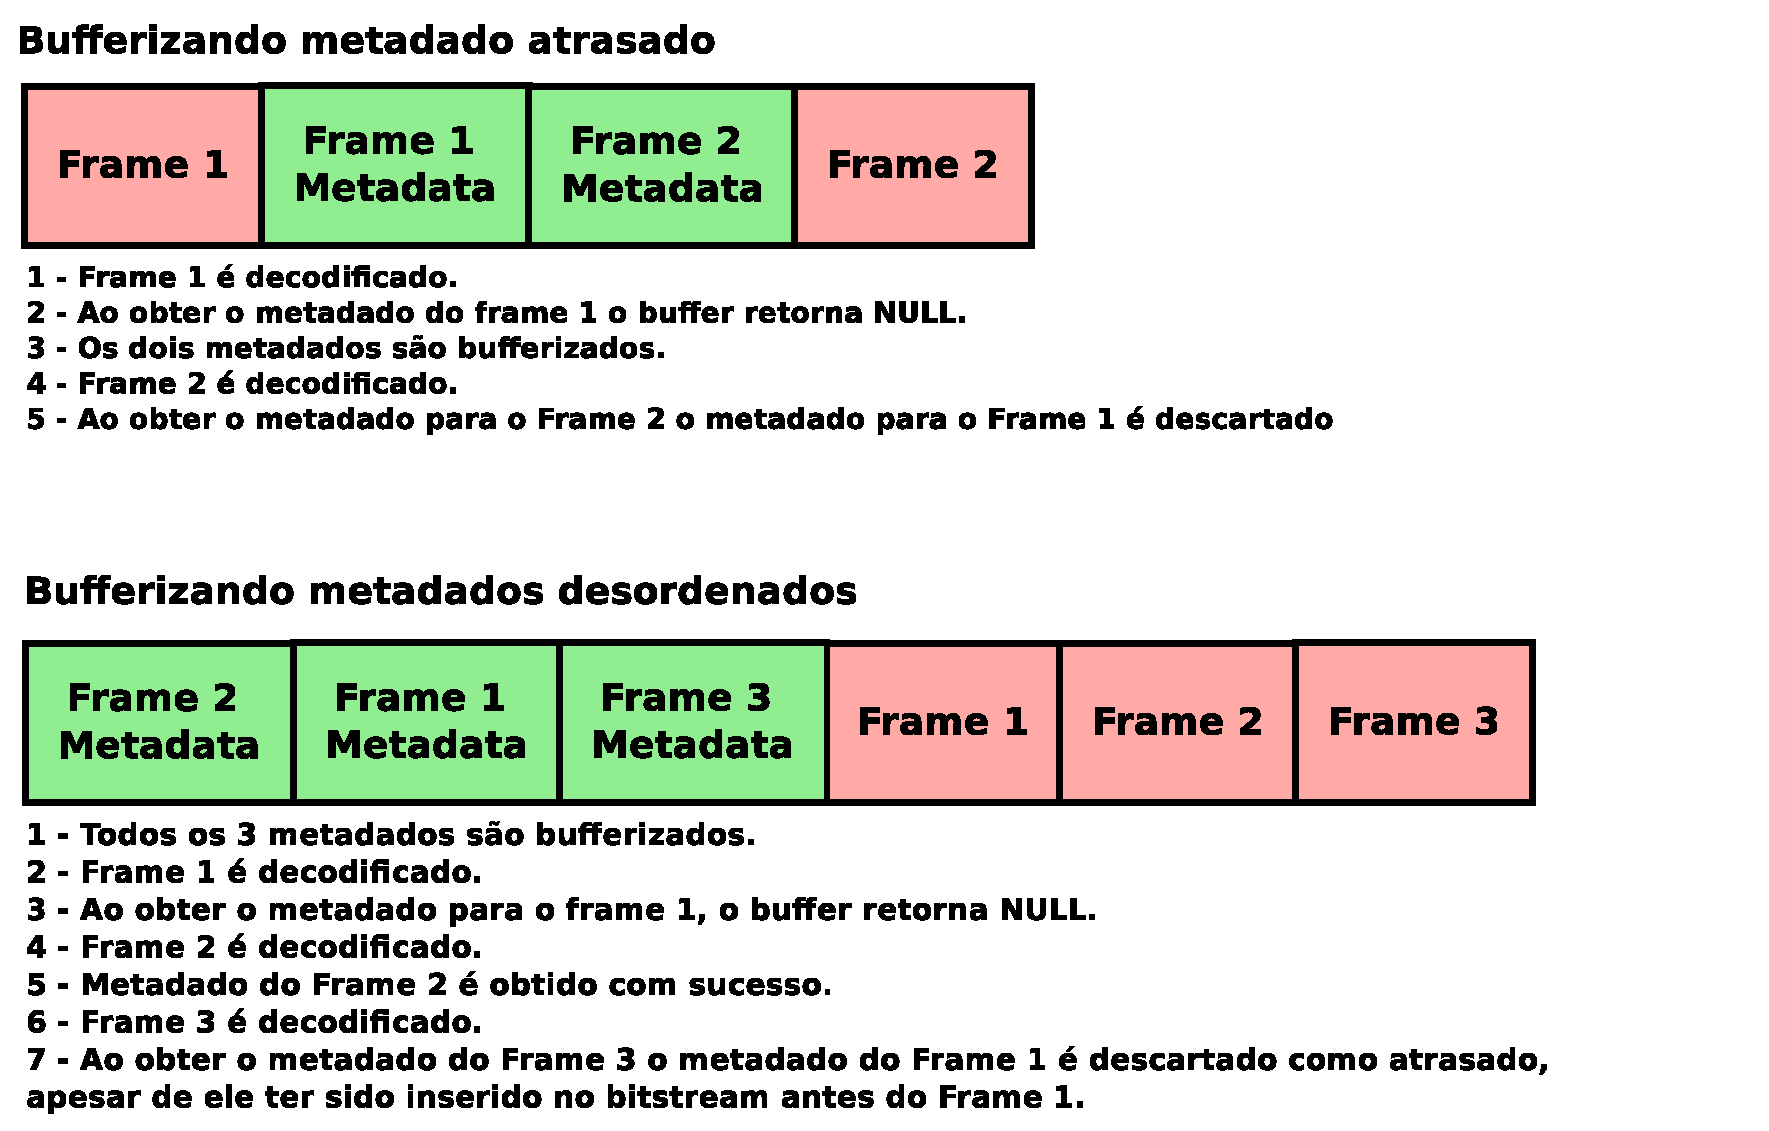
\includegraphics[scale=0.6]{imagens/fig13.eps}
\caption{Exemplo de problemas que podem ocorrer na recuperação dos metadados se eles forem inseridos de maneira errada no bitstream. Metadados em verde, quadros em vermelho.}
\label{fig:bad_metadada_ordering}
\end{figure}

A figura ~\ref{fig:bad_metadada_ordering} exemplifica alguns problemas que podem ocorrer ao bufferizar metadados que não foram inseridos no bitstream de maneira adequada.


\section{ Módulo metadata\_extractor }

Este módulo é responsável pela extração de metadados a partir de quadros brutos e das informações de estimativa de movimento fornecidas. Na atual implementação  ele pode extrair metadados do tipo \textit{ExtractedObjectBoundingBox} e \textit{ExtractedYImage}.

É escrito em linguagem C e se encontra no diretório \textit{lencod} do software de referência já que ele é utilizado tanto pelo codificador como pelo decodificador. Todas as funções são declaradas no cabeçalho \textit{lencod/inc/metadata\_extractor.h} e implementadas em \textit{lencod/src/metadata\_extractor.c}.

Nele também foi utilizada a mesma abordagem orientada a objetos utilizada no módulo \textit{extracted\_metadata} e as mesmas regras foram utilizadas para os nomes das funções que representam métodos da classe \textit{MetadataExtractor}.

O uso do classificador Haar na implementação do extrator de metadados será comentado nessa seção. A implementação completa do módulo encontra-se no apêndice C.


\subsection{ Metadata\_Extractor }

É o único objeto exportado publicamente pelo módulo e possui todo o contexto da extração de metadados. O método \textit{new} cria um novo extrator de metadados, na criação várias características do extrator podem ser configuradas por meio dos seguintes parâmetros: 

\begin{itemize}
	\item min\_width - Comprimento mínimo do objeto de interesse.
	\item min\_height - Altura mínima do objeto de interesse.
	\item search\_hysteresis - Histerese (em quadros) para realização da busca de um novo objeto de interesse.
	\item tracking\_hysteresis - Histerese (em quadros) para realizar a confirmação de que o objeto de interesse do qual está sendo feito \textit{tracking} ainda se encontra no vídeo, e corrigir possíveis erros causados pela estimativa de movimento.
        \item training\_file - Arquivo de treinamento que será utilizado ao criar o classificador Haar desse extrator. Ele define qual é o objeto de interesse.
\end{itemize}

O termo histerese tem diferentes significados de acordo com o contexto e a área em que é utilizado, pode ser utilizado na biologia, tratamento de materiais, mecânica, entre outros. No presente trabalho a histerese se refere a quantidade de quadros necessários para realizar a execução do classificador Haar, gerando um atraso configurável na detecção de um novo objeto, ou ao confirmar a existência de um objeto previamente detectado.

O método \textit{extract\_raw\_object} extrai do quadro o plano luma do objeto de interesse (se ele existir no quadro) e retorna como um objeto \textit{ExtractedMetadata}. Para realizar a extração é necessário passar os seguintes parâmetros:

\begin{itemize}
	\item extractor - Objeto \textit{MetadataExtractor}.
	\item frame\_number - Número do quadro (em ordem de apresentação) do qual será extraído o metadado.
	\item y - Plano luma, array bidimensional[y][x] de bytes, onde y vai de 0 á altura - 1 e x vai de 0 á comprimento - 1.
	\item width - Comprimento do quadro.
        \item height - Altura do quadro.
\end{itemize}

Se o objeto de interesse não se encontrar no quadro, esse método retorna \textit{NULL}. As configurações de histerese e as informações de estimativa de movimento não são utilizadas nesse método.

O método \textit{extract\_object\_bounding\_box} extrai do quadro uma caixa delimitadora que representa a área onde se encontra o objeto de interesse no quadro e retorna como um objeto \textit{ExtractedMetadata}. Para realizar a extração é necessário passar os seguintes parâmetros:

\begin{itemize}
	\item extractor - Objeto \textit{MetadataExtractor}.
	\item frame\_number - Número do quadro (em ordem de apresentação) do qual será extraído o metadado.
	\item y - Plano luma, array bidimensional[y][x] de bytes, onde y vai de 0 à altura - 1 e x vai de 0 ao comprimento - 1.
	\item width - Comprimento do quadro.
        \item height - Altura do quadro.
\end{itemize}

Se o objeto de interesse não se encontrar no quadro, esse método retorna \textit{NULL}. As configurações de histerese e as informações de estimativa de movimento são utilizadas nesse método de acordo com o estado interno do extrator. O comportamento do método depende do estado interno do extrator:

\begin{itemize}

	\item Não realizando \textit{tracking} - Será consultada a histerese de busca, se a histerese foi ultrapassada, o classificador Haar será utilizado para realizar a busca do objeto de interesse neste quadro. Se o objeto existir, o extrator cria um objeto \textit{TrackedBoundingBox} que será utilizado internamente para realizar o \textit{tracking} do objeto, passa para o estado \textit{Realizando tracking} e retorna um objeto \textit{ExtractedObjectBoundingBox}. Se o objeto não existir o extrator reinicia a histerese de busca, continua no estado atual e retorna \textit{NULL}. Se a histerese não foi ultrapassada o extrator continua no estado atual e retorna \textit{NULL}.

	\item Realizando \textit{tracking} - Será consultada a histerese de \textit{tracking}, se a histerese foi ultrapassada, o classificador Haar será utilizado para verificar se o objeto ainda se encontra no quadro atual, se o objeto não for encontrado o extrator volta ao estado \textit{Não realizando tracking} e retorna NULL. Se o objeto de interesse está no quadro o objeto \textit{TrackedBoundingBox} é atualizado de acordo com a posição encontrada pelo classificador Haar e um \textit{ExtractedObjectBoundingBox} é retornado. Se a histerese não foi ultrapassada será retornado um objeto \textit{ExtractedObjectBoundingBox} utilizando as informações de estimativa de movimento para calcular a posição atual do objeto \textit{TrackedBoundingBox}.

\end{itemize}


\begin{figure}[H]
\centering
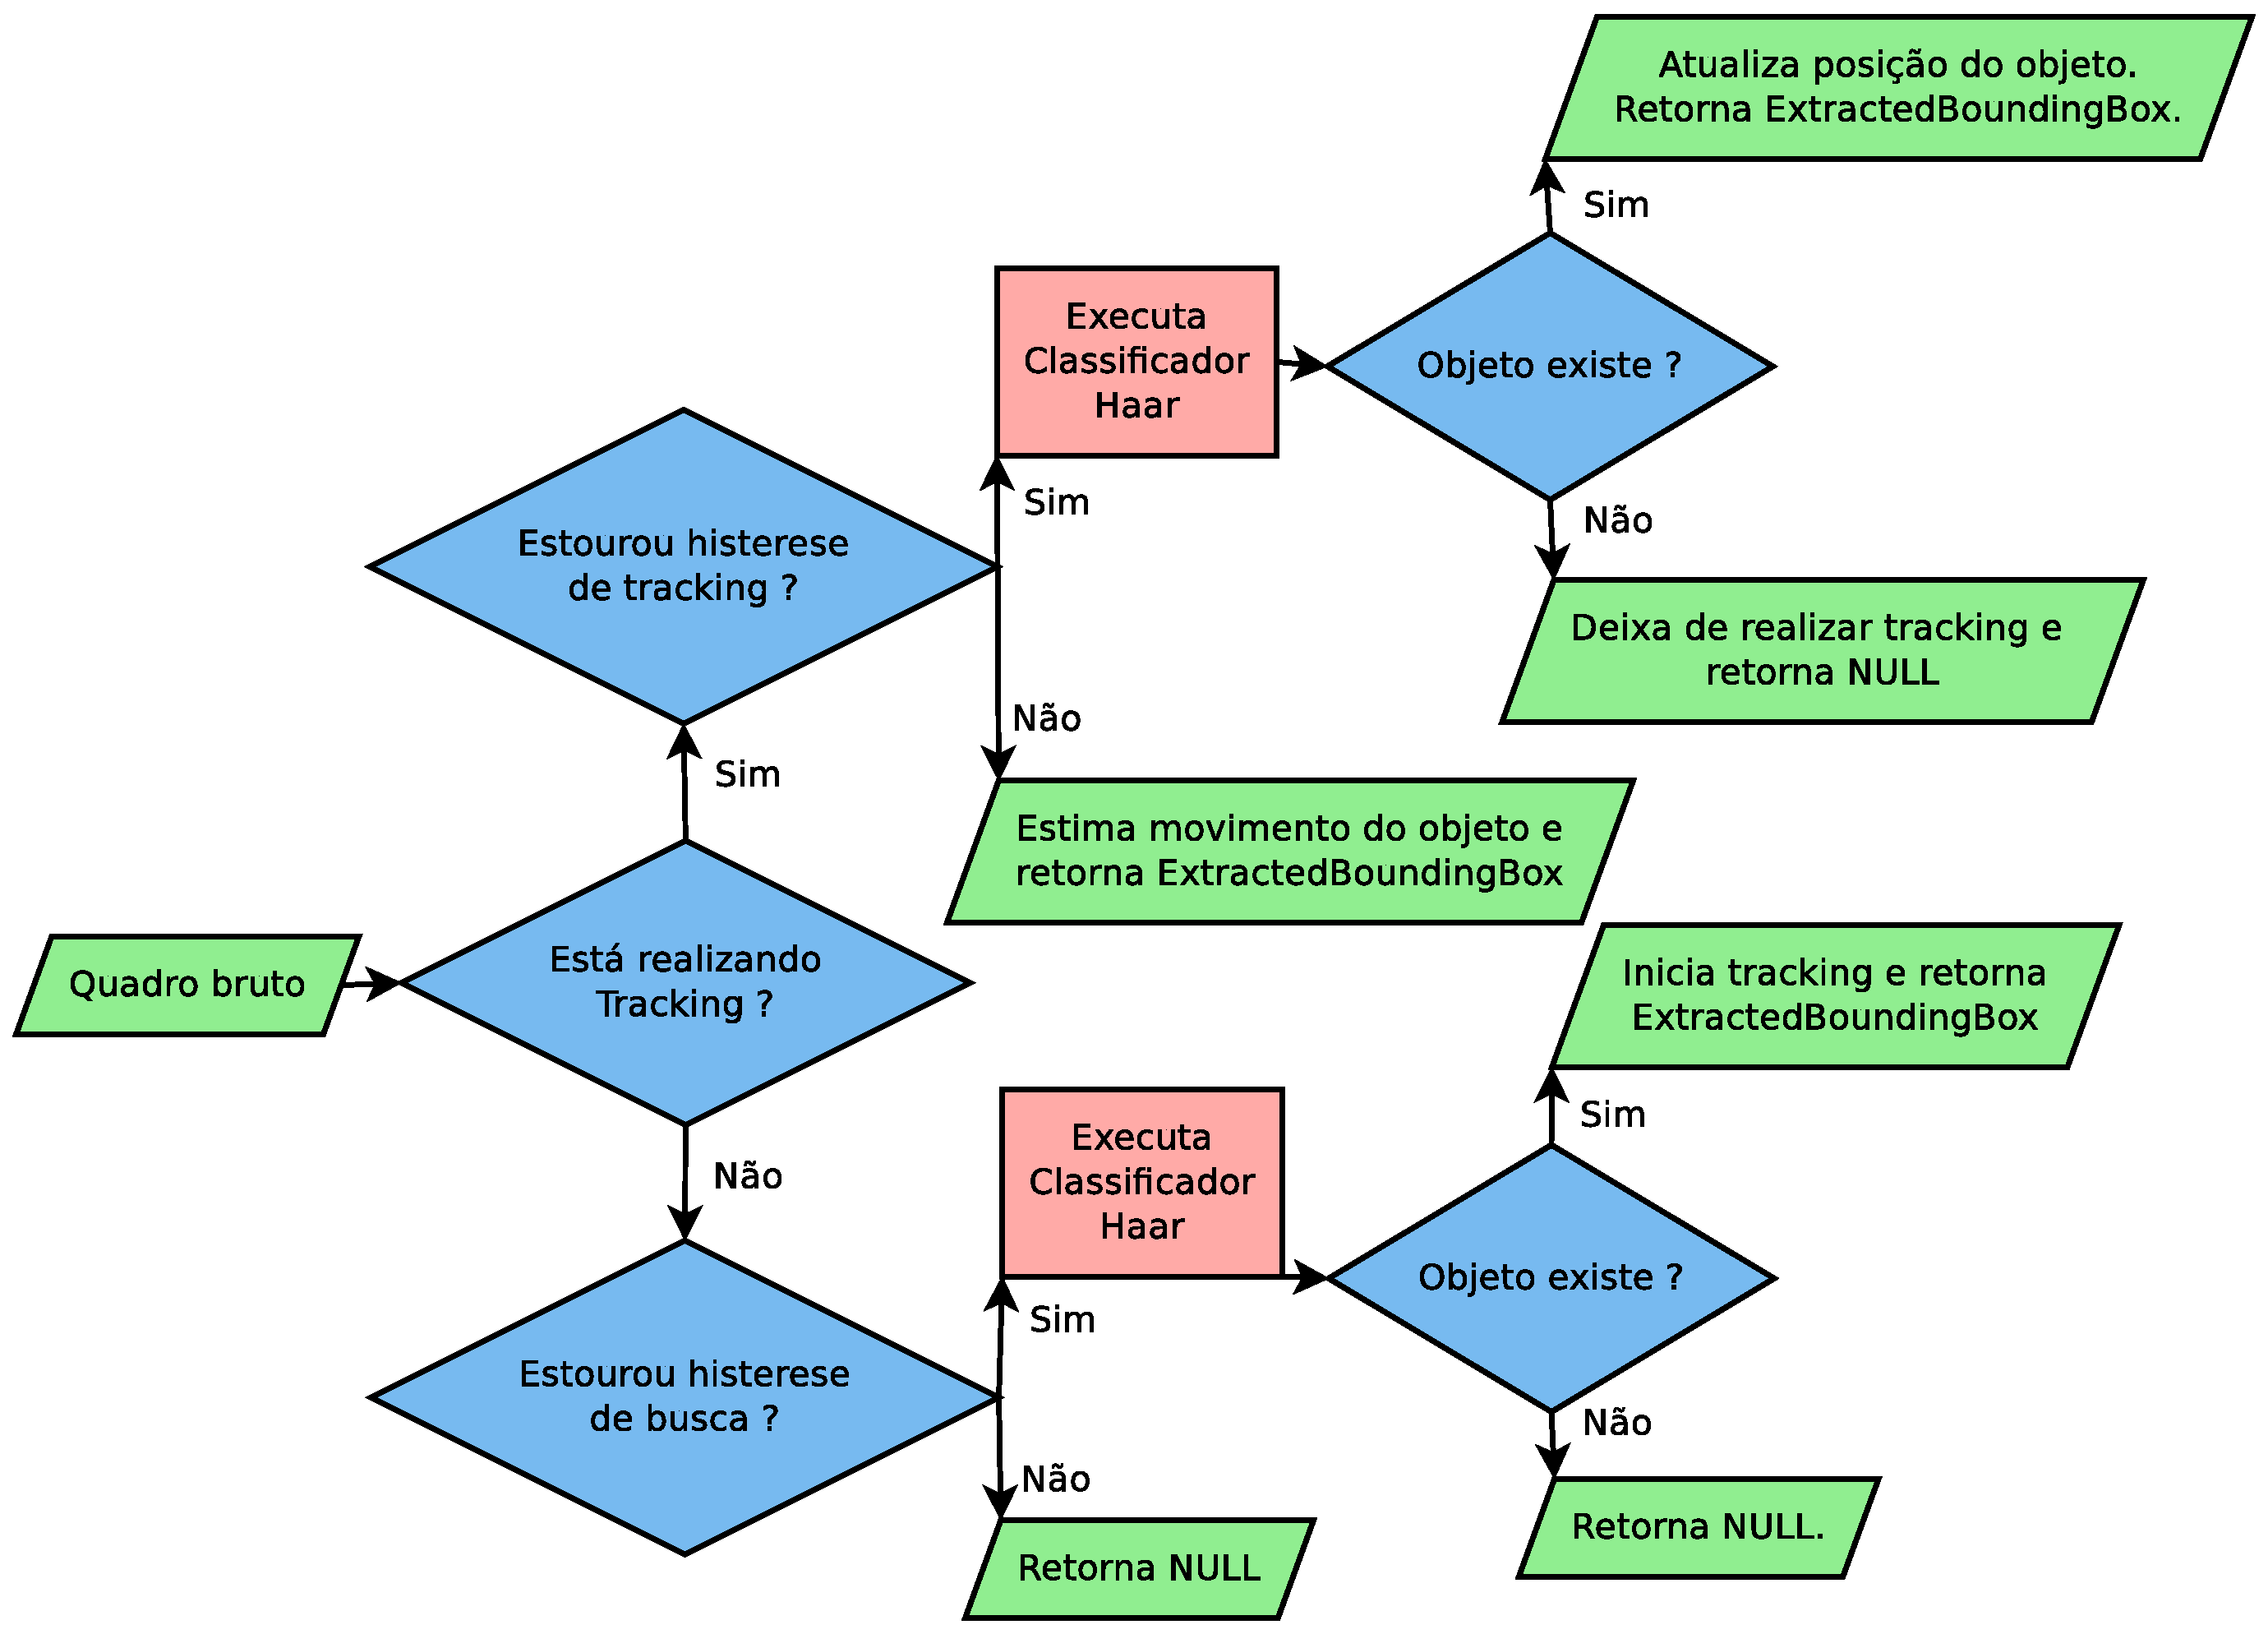
\includegraphics[scale=0.38]{imagens/fig14.eps}
\caption{Fluxograma do método extract\_object\_bounding\_box.}
\label{fig:extract_bounding_box_fluxogram}
\end{figure}

As histereses configuradas, junto com as informações de estimativa de movimento, visam utilizar os algoritmos já existentes no codificador para reduzir o custo computacional do \textit{tracking} de um objeto no vídeo. Ao invés de realizar o processamento de todos os quadros brutos no classificador Haar para realizar o \textit{tracking} do objeto ao longo do vídeo, a histerese diminui o custo computacional por atualizar a posição do objeto em intervalos fixos. Os vetores de movimento calculados pelo codificador são utilizados para suavizar o \textit{tracking}, estimando a nova posição do objeto enquanto a histerese de \textit{tracking} não estoura.

Por exemplo, em um vídeo com 300 quadros sem nenhum objeto de interesse, com uma histerese de busca de 10 quadros, o classificador Haar será chamado apenas 30 vezes, ao invés de 300 vezes. A configuração é especialmente útil em vídeos com \textit{framerate} muito alto, já que determinados objetos têm uma velocidade de locomoção esperada em um vídeo, logo não é necessário processar todos os quadros.

\begin{figure}[H]
\centering
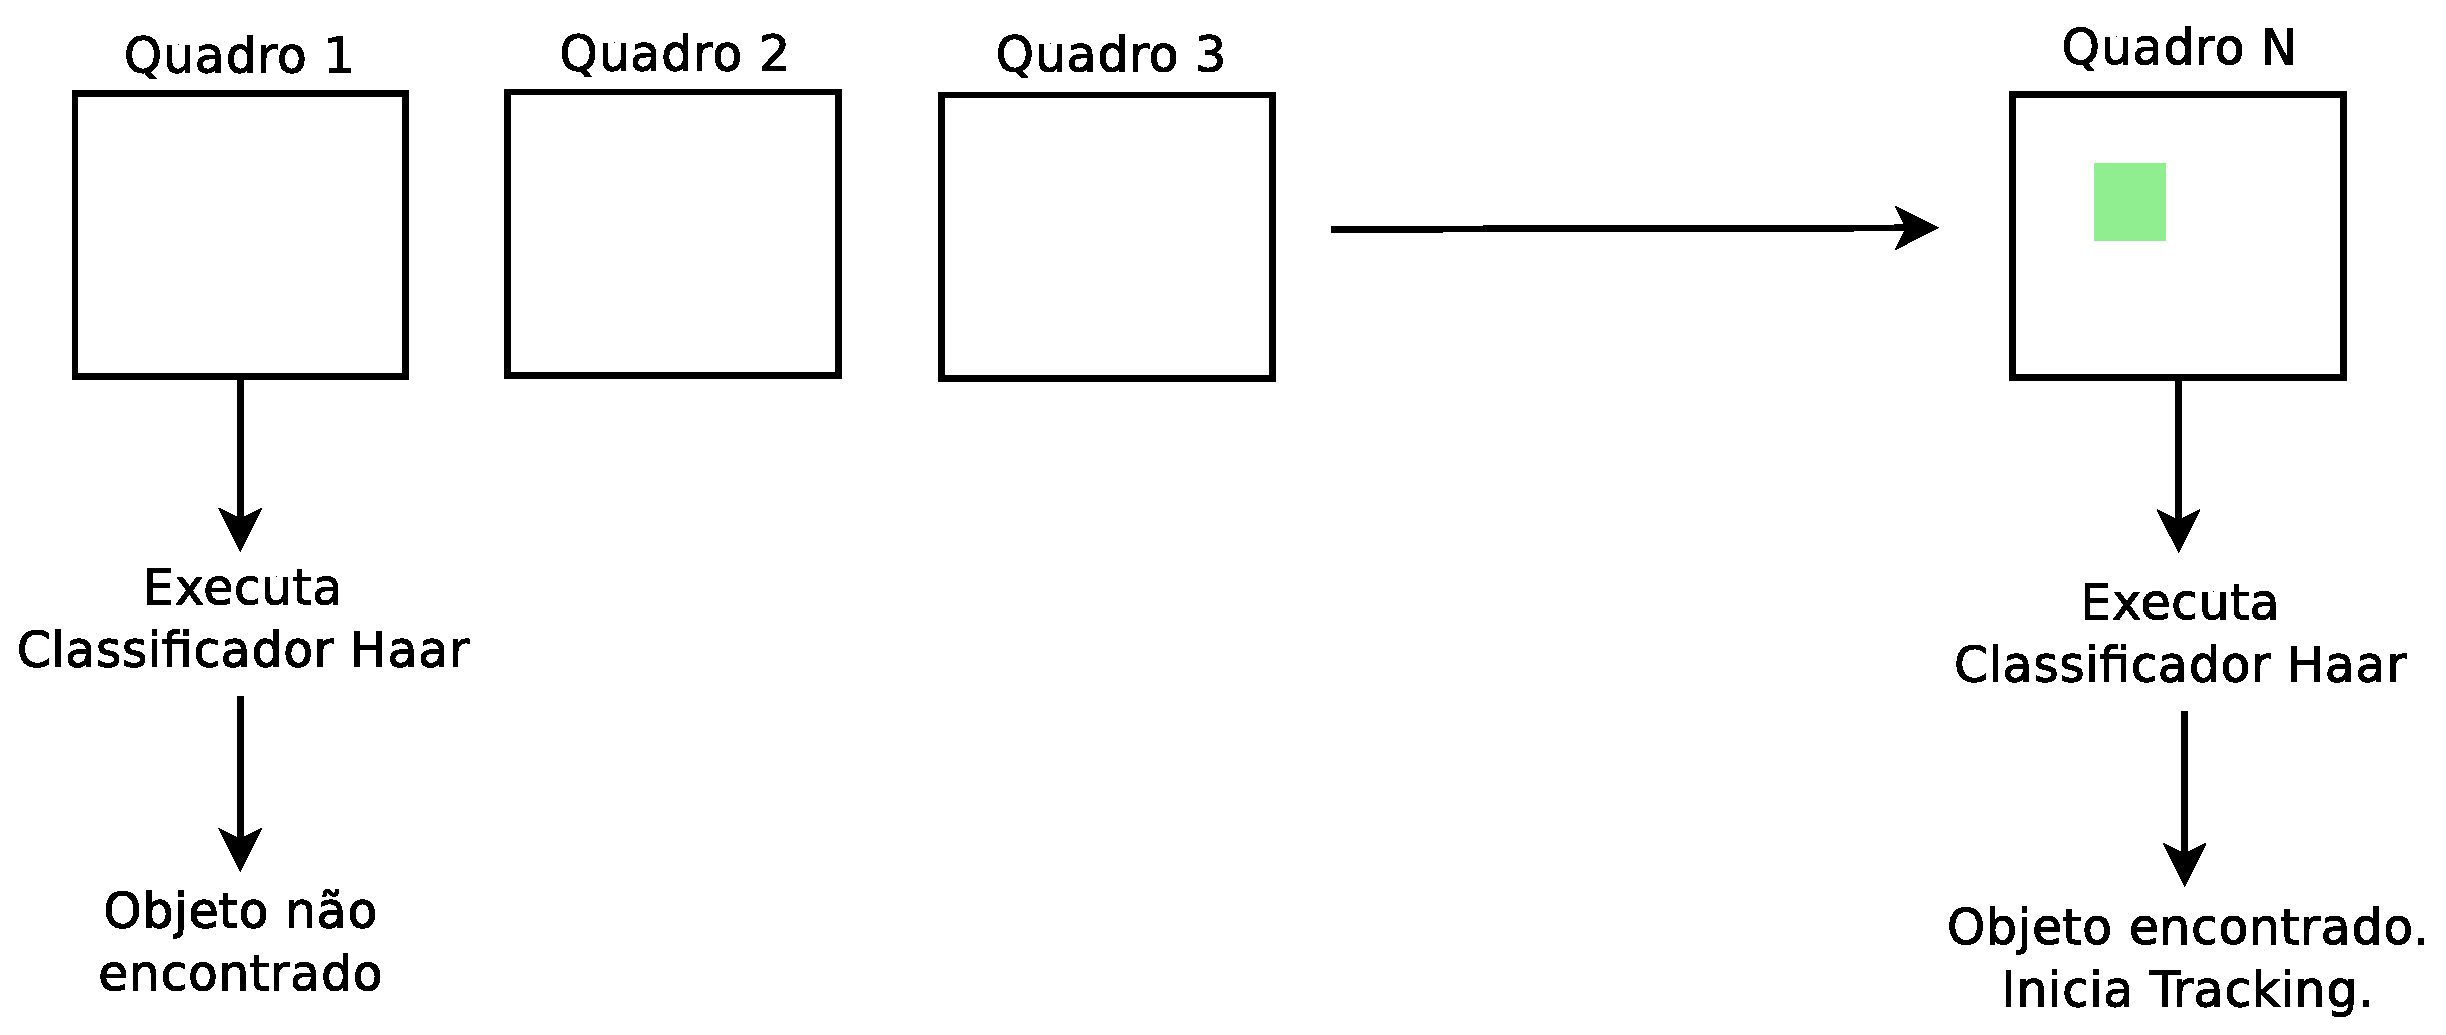
\includegraphics[scale=0.4]{imagens/fig23.eps}
\caption{Exemplo do funcionamento da histerese de busca.}
\label{fig:search_histeresys_example}
\end{figure}

O mesmo se dá quando o objeto já foi detectado, não é necessário executar o classificador em todos os quadros, os vetores de estimativa de movimento nos dão uma ideia aproximada da posição do objeto, até que seja alcançada a histerese de \textit{tracking}.

\begin{figure}[H]
\centering
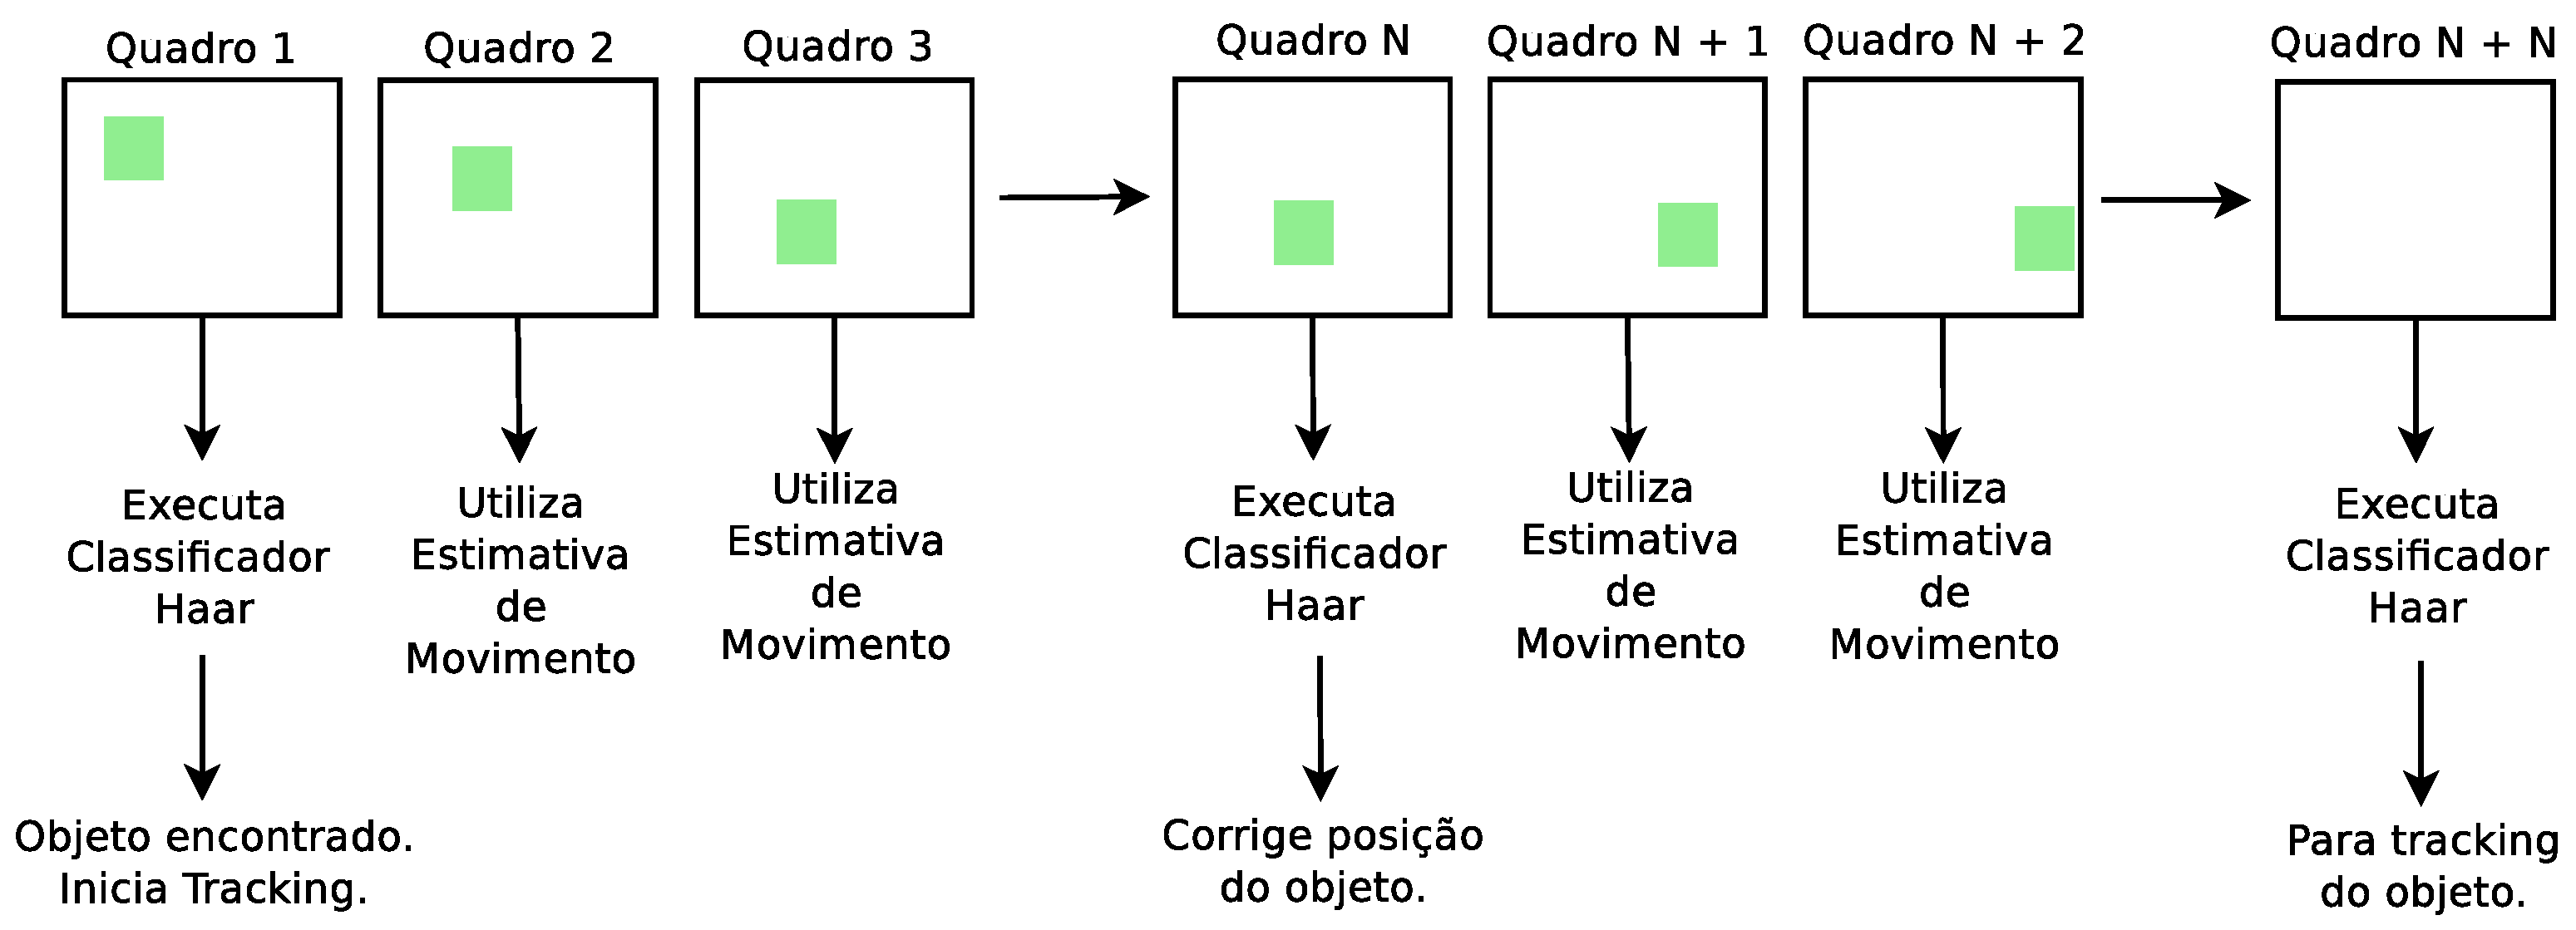
\includegraphics[scale=0.3]{imagens/fig24.eps}
\caption{Exemplo do funcionamento da histerese de \textit{tracking}.}
\label{fig:tracking_histeresys_example}
\end{figure}

Cada extrator só pode realizar a monitoração de um objeto de interesse, se existirem diversos objetos de interesse no quadro ele irá detectar apenas um e realizar o \textit{tracking} desse objeto. Criar vários extratores para detectar o mesmo tipo de objeto geraria problemas como detectar várias vezes o mesmo objeto, mas seria possível criar vários extratores para detectar objetos diferentes e utilizá-los em paralelo.


\subsection{ Utilizando o classificador Haar }


O classificador Haar foi escolhido como algoritmo de detecção de padrões a ser utilizado nesse trabalho. Como ele ficou completamente oculto na implementação do módulo \textit{metadata\_extractor} é possível alterar a implementação do módulo, utilizando outro algoritmo de detecção de padrões, sem realizar qualquer alteração na API pública do módulo, ou simplesmente removê-lo. A única limitação da API atual é que ela trabalha apenas com as informações de luminância, para trabalhar com algoritmos que utilizem informações de cor será necessária uma alteração na API do módulo atual.

A implementação do classificador Haar do OpenCV foi escolhida para realizar a detecção de objetos por ser bem documentada e fácil de utilizar, sem contar que o OpenCV já dispõe de uma série de outras funções que facilitam trabalhar com o quadro bruto. Outra vantagem é que ele trabalha com imagens em escala de cinza, independente da configuração do vídeo bruto o plano de luminância sempre possui a maior resolução possível. Técnicas que utilizam informações de cor teriam a desvantagem de ter de trabalhar com informações de cor com resolução reduzida. 

Outra motivação é a possibilidade de acelerar o classificador Haar diretamente em hardware, como pode ser visto em  \cite{haarFPGA}, onde a parte mais complexa do classificador Haar (90\% do tempo de processamento) foi implementando em hardware, o que se alinha com a ideia de construir um chip codificador H.264 com detecção de objetos integrada em tempo real. 

A principal função que é utilizada na detecção de um objeto é \textit{cvHaarDetectObjects( const CvArr* image, CvHaarClassifierCascade* cascade, CvMemStorage* storage, double scale\_factor, int min\_neighbors, int flags, CvSize min\_size)}.

O primeiro parâmetro é a imagem onde será realizada a busca, em escala de cinza, que será obtida através do plano luma original do codificador. O segundo parâmetro é o classificador que é criado no método \textit{new} do objeto \textit{MetadataExtractor}. O terceiro parâmetro é o buffer de trabalho do classificador que também é criado no método \textit{new}. 

O classificador busca pelo objeto de interesse em todas as escalas possíveis, o quarto parâmetro significa o quão grande será o pulo entre cada escala, um valor alto vai tornar o classificador mais rápido porém aumentará as chances de falso negativo. O quinto parâmetro é um controle para prevenir falsos positivos. Na área onde se encontra o objeto de interesse costuma ocorrer várias detecções com sucesso para o mesmo objeto, já que os pixels ao redor da área e em escalas diferentes indicam que existe o objeto de interesse. Por exemplo, o valor 3 indica que o classificador só considerará o objeto como presente se ocorrerem 3 detecções sobrepostas na mesma área.

O sexto parâmetro são as flags do processo de busca, existem 4 flags que podem ser compostas com o operador OR:

\begin{itemize}
	\item CV\_HAAR\_DO\_CANNY\_PRUNING - Fará com que regiões planas da imagem (sem linhas) sejam ignoradas.    
	\item CV\_HAAR\_SCALE\_IMAGE - Faz com que o classificador escalone a imagem em vez de escalonar ele mesmo.
	\item CV\_HAAR\_FIND\_BIGGEST\_OBJECT - Faz com que o classificador retorne apenas o maior objeto detectado (se houver mais de um).
	\item CV\_HAAR\_DO\_ROUGH\_SEARCH - Só pode ser utilizado em conjunto com a flag CV\_HAAR\_FIND\_BIGGEST\_OBJECT, faz com que o classificador encerre a busca assim que ele encontrar o objeto de interesse (nesse caso o maior).
\end{itemize}

O sétimo parâmetro é o tamanho mínimo que o objeto deve possuir para ser detectado pelo classificador. Quanto maior for o tamanho mínimo mais rápido o classificador irá executar, mas maior será a possibilidade de ocorrer falso negativo.


\subsection{ Realizando estimativa de movimento }

A estimativa de movimento de um objeto é realizada por um trabalho em conjunto entre o método \textit{extract\_object\_bounding\_box} e o método \textit{add\_motion\_estimation\_info}. Um \textit{MetadataExtractor} recebe as informações de estimativa de movimento através do método \textit{add\_motion\_estimation\_info}, essas informações por sua vez serão utilizadas na execução do método \textit{extract\_object\_bounding\_box}. O método \textit{add\_motion\_estimation\_info} recebe os seguintes parâmetros:

\begin{itemize}
	\item extractor - Objeto \textit{MetadataExtractor}.
        \item block\_x - X do bloco, em coordenada de bloco.
        \item block\_y - Y do bloco, em coordenada de bloco.
        \item x\_motion\_estimation - Estimativa de movimento para a coordenada x do bloco.
        \item y\_motion\_estimation - Estimativa de movimento para a coordenada y do bloco.
\end{itemize}

Se o extrator não estiver realizando \textit{tracking} de um objeto a chamada para este método é ignorada. Se o extrator está realizando \textit{tracking}, será avaliado se este bloco faz parte da caixa delimitadora (representada pela classe \textit{TrackedBoundingBox}) do objeto de interesse. Se qualquer parte do bloco estiver dentro da caixa delimitadora, as informações de estimativa de movimento dele serão utilizadas para estimar o movimento da caixa delimitadora do objeto de interesse.

Essa abordagem é eficiente já que bastam algumas comparações bem simples para verificar se a área do bloco tem uma interseção com a área da caixa delimitadora do objeto de interesse, porém a caixa delimitadora nem sempre representa perfeitamente o objeto (o objeto teria de ter a forma de uma caixa também), dessa maneira acaba-se utilizando a estimativa de movimento de blocos que fazem parte da caixa delimitadora mas não do objeto, gerando um erro que se acumula a cada estimativa de movimento do objeto. Isso limita o uso da técnica, sendo necessária uma histerese de \textit{tracking} pequena dependendo do quanto o objeto se movimenta e da sua caixa delimitadora.

No software de referência utiliza-se um modelo simplificado de estimativa de movimento, o tamanho dos blocos utilizados na estimativa de movimento sempre possuem um tamanho de 4 x 4 pixels, independente do modo escolhido. Dessa maneira para obter as coordenadas reais do bloco basta multiplicar as coordenadas do bloco por 4. Tendo as coordenadas reais do bloco fica fácil determinar se o bloco está dentro ou não da caixa delimitadora do objeto de interesse.


\begin{figure}[H]
\centering
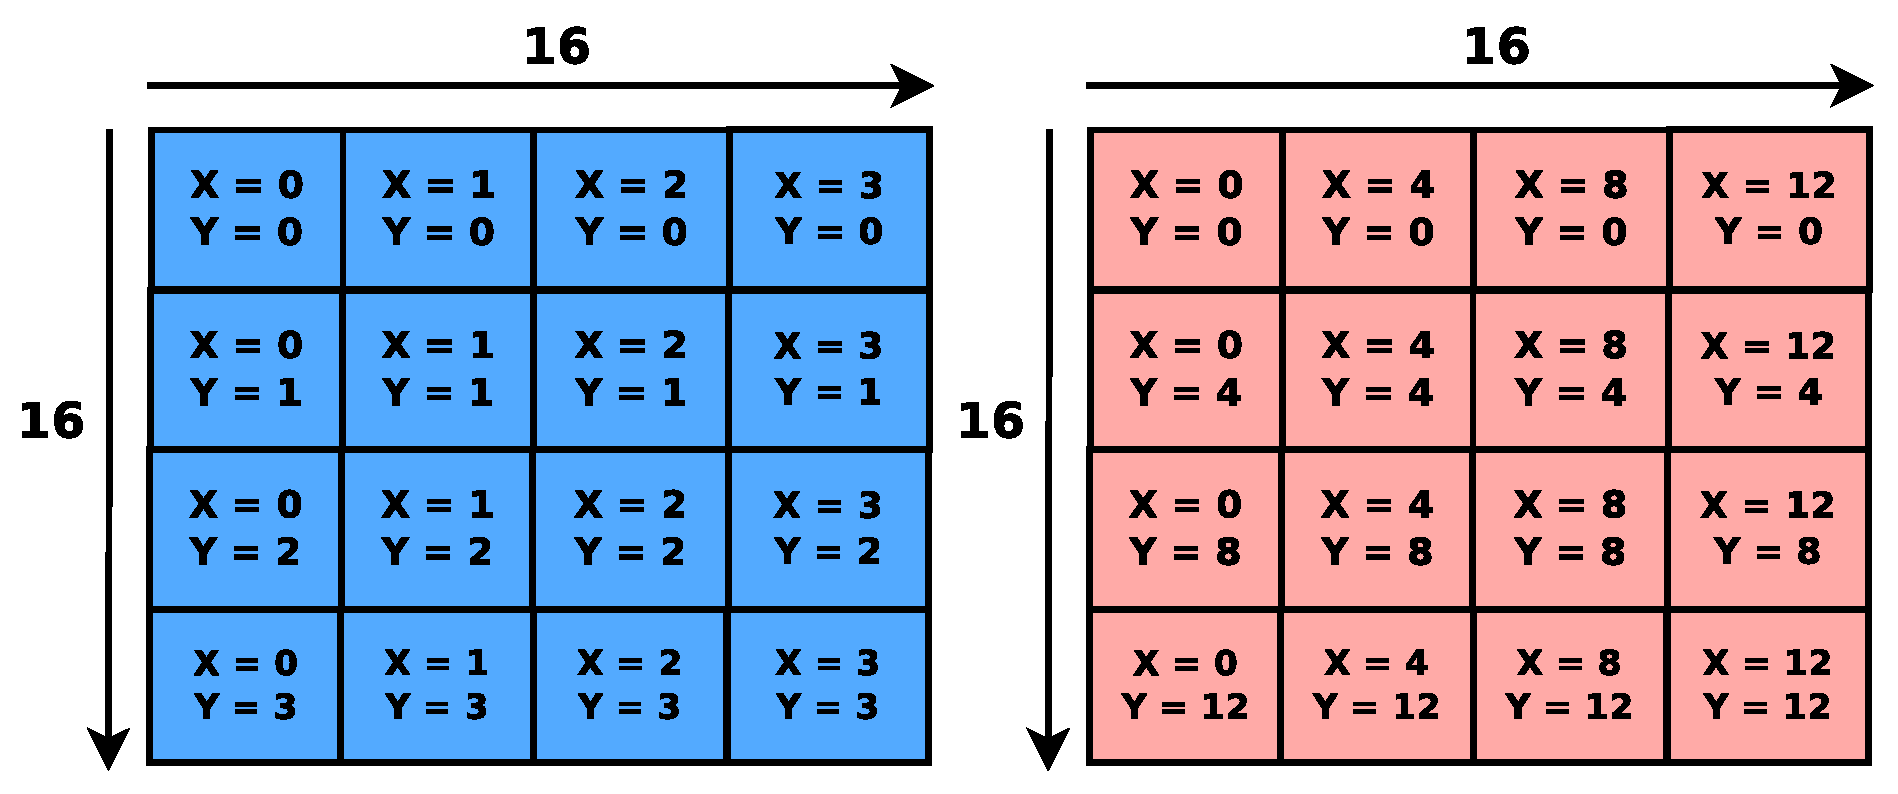
\includegraphics[scale=0.4]{imagens/fig16.eps}
\caption{Comparação entre as coordenadas dos blocos (em azul) da estimativa de movimento e as coordenadas reais (em vermelho) que elas representam.}
\label{fig:block_coordinate_example}
\end{figure}


É importante ressaltar que o tamanho fixo 4 x 4 para os blocos da estimativa de movimento não é verdade para todos os codificadores. Alguns codificadores possuem uma hierarquia e seria necessário derivar a estimativa de movimento para um bloco dependendo do modo utilizado.

O valor da estimativa de movimento é informado em unidades de QPel (Quarter Pel refinement), onde um quarto das amostras são sub-amostras interpoladas, causadas por frações de vetores de movimento.  Mais detalhes a respeito desse processo podem ser encontrados em \cite{ituh264avc} subcláusula 8.4.2.2. Um vetor x negativo indica um movimento para a direita, y negativo indica um movimento para baixo, x positivo indica um movimento para a esquerda e um y positivo um movimento para cima.


\begin{figure}[H]
\centering
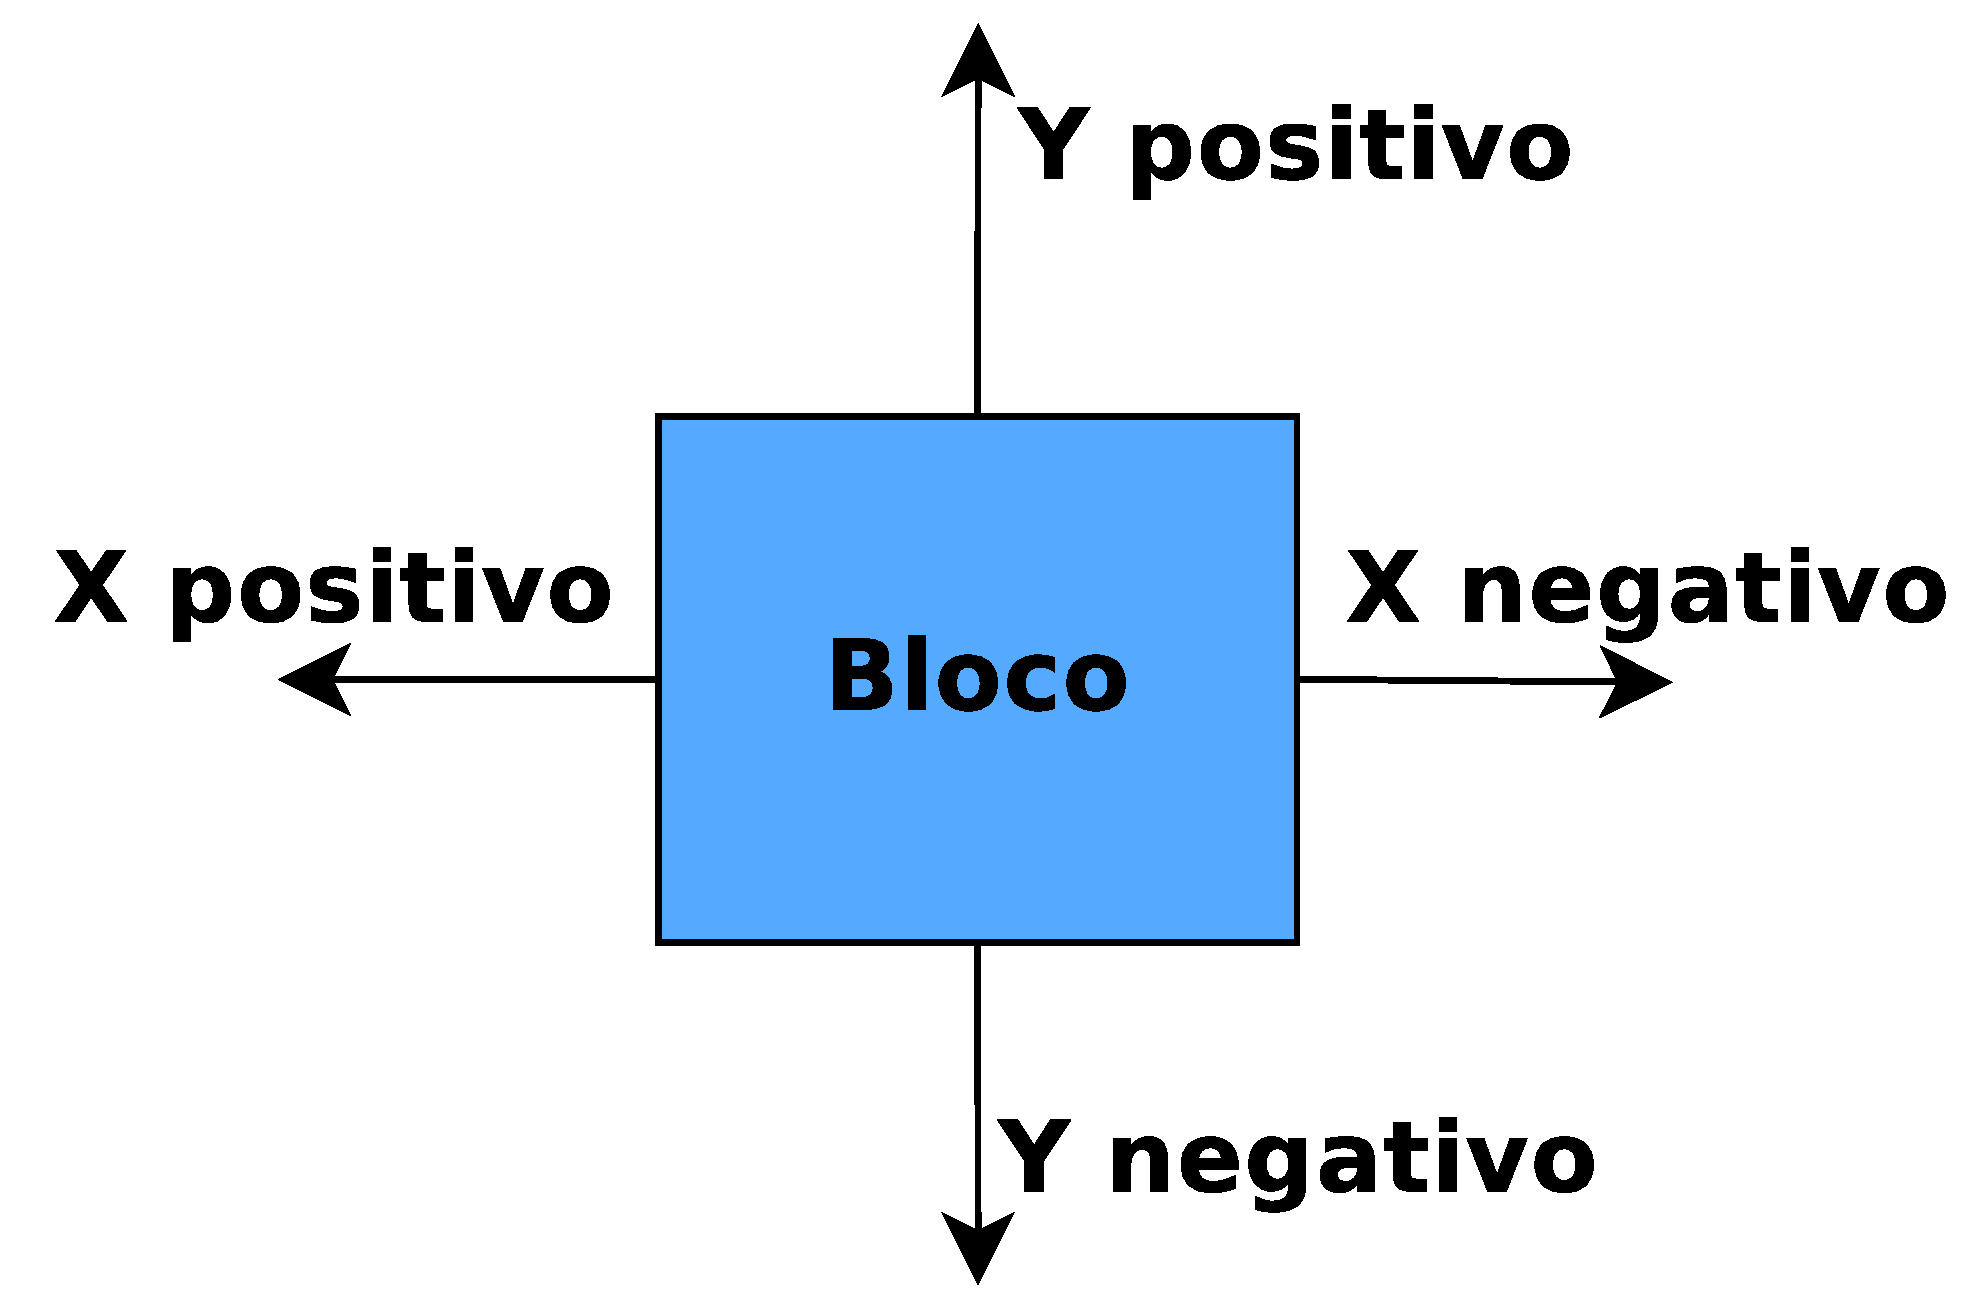
\includegraphics[scale=0.3]{imagens/fig15.eps}
\caption{Como os vetores de movimento de um bloco representam a sua movimentação no vídeo.}
\label{fig:block_vector_example}
\end{figure}


Todas as informações relativas a estimativa de movimento do objeto de interesse são guardadas no \textit{TrackedBoundingBox}, essa classe representa a caixa delimitadora do objeto de interesse do qual está sendo feito o \textit{tracking}, e é criada quando se identifica um objeto de interesse pela primeira vez. Nele é guardado um somatório de todos os vetores (em QPel) de movimento alimentados no extrator. Ao chamar o método \textit{extract\_object\_bounding\_box} no estado de \textit{tracking}, serão utilizadas as informações contidas no \textit{TrackedBoundingBox} para realizar a estimativa de movimento do objeto.

Nesse método é realizada a média aritmética simples de todos os vetores, ou seja o somatório de todos os vetores é dividido pela quantidade de blocos que foram utilizados para realizar a estimativa de movimento. O somatório de todos os vetores é dividido por 4 antes de ser dividido pela quantidade de blocos, pois o somatório dos vetores está em unidades de QPel. Realizar essa divisão por 4 nos fornece a estimativa de movimento em pixels. 

Tendo a estimativa de movimento em pixels basta subtrair a estimativa das coordenadas da \textit{TrackedBoundingBox}. Essas novas coordenadas serão utilizadas para criar o \textit{ExtractedObjectBoundingBox} que é retornado. As coordenadas (x,y) são guardadas como double no \textit{TrackedBoundingBox} para que não ocorra perda de precisão no acúmulo de pequenos movimentos, como pode ser visto na figura ~\ref{fig:object_motion_estimation_example}. 


\begin{figure}[H]
\centering
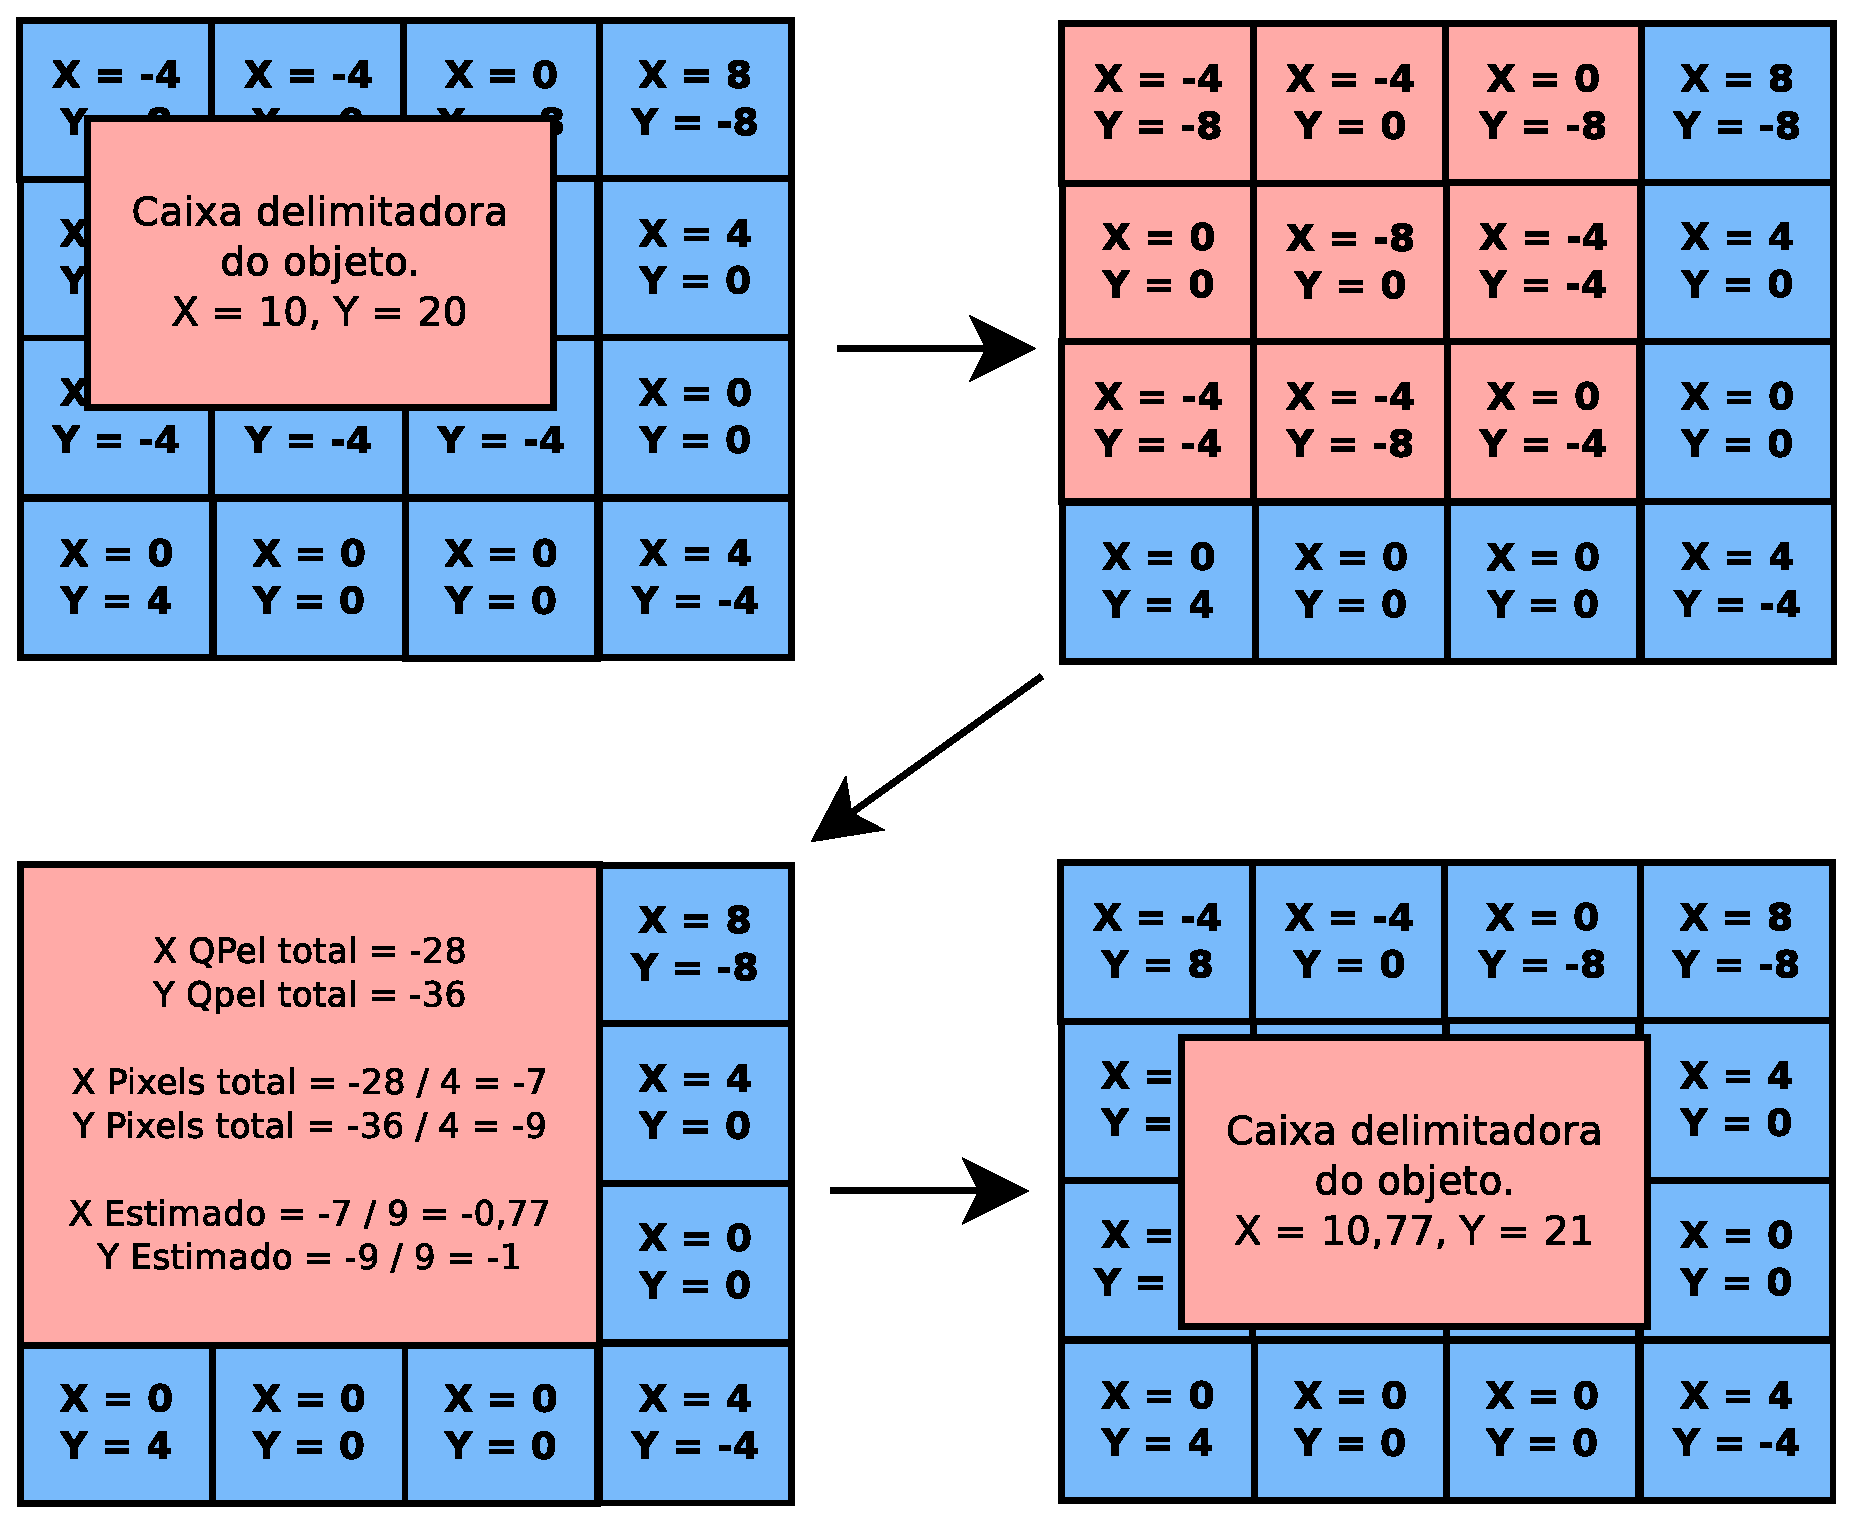
\includegraphics[scale=0.45]{imagens/fig17.eps}
\caption{Estimativa de movimento de um objeto.}
\label{fig:object_motion_estimation_example}
\end{figure}


Esse processo pode ser visto em detalhes no método \textit{estimate\_motion} da classe \textit{TrackedBoundingBox} que se encontra implementado em \textit{/lencod/src/metadata\_extractor.c}. 


\section{ Alterações realizadas no codificador }


O objetivo da criação dos módulos \textit{metadata\_extractor} e \textit{extracted\_metadata} foi reduzir ao máximo as alterações que teriam de ser realizadas no codificador e no decodificador e desacoplando o processo de extração de metadados do software de referência. Isso facilita a possibilidade de portar o sistema de detecção e \textit{tracking} de objetos para uma outra implementação do H264.

Nesta seção serão apresentadas as alterações realizadas no codificador do software de referência, para integrá-lo com os módulos construídos. As alterações realizadas no codificador se encontram no anexo A.


\begin{figure}[H]
\centering
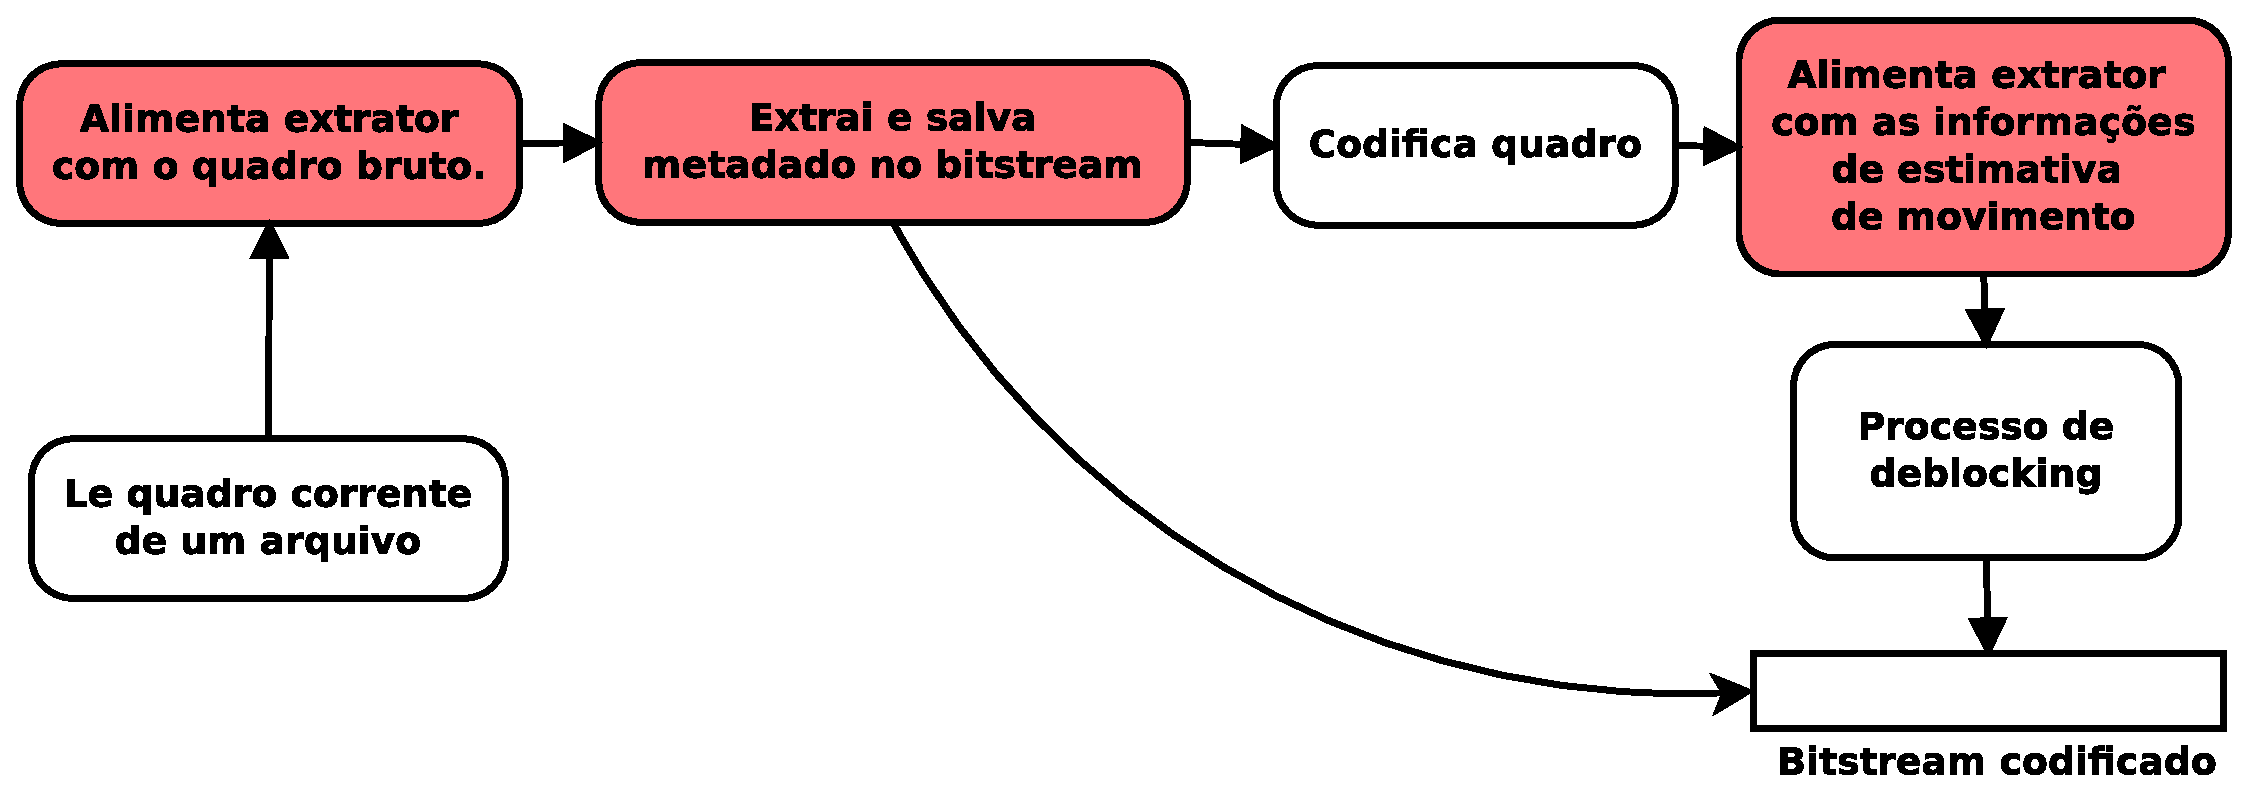
\includegraphics[scale=0.45]{imagens/fig18.eps}
\caption{Visão geral do codificador H.264 modificado. Os blocos vermelhos representam os processos adicionados ao codificador.}
\label{fig:h264_moded_encoder}
\end{figure}


\subsection{ Processando o quadro bruto }

Para extrair metadados do quadro bruto antes de ocorrer o processo de codificação, foi necessário primeiro descobrir qual o melhor local dentro do codificador para se obter o quadro que vai ser codificado. No caso do software de referência utilizado neste trabalho a entrada de dados é feita por arquivo. Foi necessário estudar quando o codificador lê o quadro e como ele organiza este quadro na memória.

A partir da função \textit{main} em \textit{lencod/src/lencod.c}, analisando como o codificador procedia para codificar os quadros, foi encontrada uma chamada para a função \textit{encode\_one\_frame}, esta função é implementada no módulo \textit{lencod/src/image.c}, é nesta função que o quadro é carregado em memória e pré-processado.

Dentro da função \textit{encode\_one\_frame}, o processamento do quadro bruto é realizado logo após a chamada de função \textit{process\_image}, que realiza o processamento final em cima do quadro bruto, antes de se iniciar a codificação dele. É neste ponto que o método \textit{extract\_object\_bounding\_box} é chamado e o metadado extraído é salvo no bitstream na forma de mensagem SEI \textit{Unregistered Userdata}, utilizando o módulo \textit{udata\_gen}.

\begin{lstlisting}

process_image(p_Vid, p_Inp);

if (p_Inp->object_detection_enable) {
    
  ExtractedMetadata * metadata = metadata_extractor_extract_object_bounding_box(p_Vid->metadata_extractor, p_Vid->frame_no, (unsigned char **) p_Vid->imgData.frm_data[0], p_Vid->imgData.format.width[0], p_Vid->imgData.format.height[0]);

  if (metadata) {
    int size                = extracted_metadata_get_serialized_size(metadata);
    char * data             = malloc(size);
    NALU_t * nalu           = NULL;
     
    /* Serialize the metadata */
    extracted_metadata_serialize(metadata, data);
      
    /* Insert the serialized metadata on the bitstream as SEI NALU. */
    nalu = user_data_generate_unregistered_sei_nalu(data, size);
    p_Vid->WriteNALU (p_Vid, nalu);

    FreeNALU (nalu);
    free(data);
    extracted_metadata_free(metadata);
  }

}

pad_borders (p_Inp->output, p_Vid->width, p_Vid->height, p_Vid->width_cr, p_Vid->height_cr, p_Vid->imgData.frm_data);

\end{lstlisting}

Tendo encontrado um bom lugar para extrair as informações foi necessário entender como o quadro fica organizado na memória. A estrutura \textit{ImageData} armazena as informações de um quadro, e o quadro original é carregado no campo \textit{imgdata} da estrutura \textit{VideoParameters}. A definição da estrutura \textit{ImageData} se encontra no módulo \textit{lcommon/inc/io\_image.h} e a estrutura \textit{VideoParameters} é definida em \textit{lencod/inc/global.h}.

O quadro original carregado se encontra no campo \textit{frm\_data} da estrutura \textit{ImageData}:

\begin{lstlisting}

typedef struct image_data
{
  FrameFormat format;               //!< image format
  // Standard data
  imgpel **frm_data[MAX_PLANE];     //!< Frame Data
  imgpel **top_data[MAX_PLANE];     //!< pointers to top field data
  imgpel **bot_data[MAX_PLANE];     //!< pointers to bottom field data

  //! Optional data (could also add uint8 data in case imgpel is of type uint16)
  //! These can be useful for enabling input/conversion of content of different types
  //! while keeping optimal processing size.
  uint16 **frm_uint16[MAX_PLANE];   //!< optional frame Data for uint16
  uint16 **top_uint16[MAX_PLANE];   //!< optional pointers to top field data
  uint16 **bot_uint16[MAX_PLANE];   //!< optional pointers to bottom field data

  int frm_stride[MAX_PLANE];
  int top_stride[MAX_PLANE];
  int bot_stride[MAX_PLANE];
} ImageData;

\end{lstlisting}

Este campo é um array tri-dimensional de \textit{imgpel}, o tipo \textit{imgpel} representa o tamanho de cada pixel e é definido no módulo \textit{lcommon/inc/typedefs.h}:

\begin{lstlisting}

#if (IMGTYPE == 0)
typedef byte   imgpel;           //!< pixel type
typedef uint16 distpel;          //!< distortion type (for pixels)
typedef int32  distblk;          //!< distortion type (for Macroblock)
typedef int32  transpel;         //!< transformed coefficient type
#elif (IMGTYPE == 2)
typedef float imgpel;
typedef float distpel;
typedef float distblk;
typedef int32 transpel;
#else
typedef uint16 imgpel;
typedef uint32 distpel;
typedef int64  distblk;
typedef int32  transpel;
#endif

\end{lstlisting}

\textit{IMGTYPE} é o que define o tamanho do pixel, e pode ser definido tanto para o codificador como para o decodificador (cada um deles pode trabalhar com um tamanho de pixel diferente). No encoder a definição do \textit{IMGTYPE} se encontra em \textit{lencod/inc/defines.h} e do decodificador em \textit{ldecod/inc/defines.h}. Por padrão o software de referência vem com esse valor definido como 1, ou seja utiliza 16 bits para representar cada pixel.

Tanto o encoder como o decodificador foram alterados para trabalhar com 8 bits para representar cada pixel, já que utilizar 16 bits não trazia vantagem alguma na extração dos metadados, gerando um overhead desnecessário.

\textit{MAX\_PLANE} é o que define a quantidade de planos existentes no quadro, e pode ser definido tanto para o encoder como para o decodificador (cada um deles pode possuir uma quantidade de planos diferente). No encoder a definição do \textit{MAX\_PLANE} se encontra em \textit{lencod/inc/defines.h} e no decodificador em \textit{ldecod/inc/defines.h}. Por padrão o software de referência vem com esse valor definido como 3, ou seja existem 3 planos em cada quadro.

Normalmente existem duas maneiras de se representar uma imagem: intercalada e planar. No caso dos quadros carregados no software de referência a representação é planar, no array tridimensional a primeira dimensão é o plano, \textit{frm\_data[0]} é o plano Y, \textit{frm\_data[1]} é o plano U e \textit{frm\_data[2]} é o plano V.

A segunda dimensão é o y/vertical do plano. A terceira dimensão é o x/horizontal do plano. O comprimento e a altura de cada plano se encontra no campo \textit{format} da estrutura \textit{ImageData}, que é do tipo \textit{FrameFormat}. O índice 0 acessa o comprimento e altura do plano Y, o índice 1 acessa o comprimento e altura dos planos de cor (UV),  o tipo \textit{FrameFormat} é definido em \textit{lcommon/inc/frame.h}:

\begin{lstlisting}

typedef struct frame_format
{
  ColorFormat yuv_format;                    //!< YUV format (0=4:0:0, 1=4:2:0, 2=4:2:2, 3=4:4:4)
  ColorModel  color_model;                   //!< 4:4:4 format (0: YUV, 1: RGB, 2: XYZ)
  double      frame_rate;                    //!< frame rate
  int         width[3];                      //!< component frame width
  int         height[3];                     //!< component frame height    
  int         auto_crop_right;               //!< luma component auto crop right
  int         auto_crop_bottom;              //!< luma component auto crop bottom
  int         auto_crop_right_cr;            //!< chroma component auto crop right
  int         auto_crop_bottom_cr;           //!< chroma component auto crop bottom
  int         width_crop;                    //!< width after cropping consideration
  int         height_crop;                   //!< height after cropping consideration
  int         mb_width;                      //!< luma component frame width
  int         mb_height;                     //!< luma component frame height    
  int         size_cmp[3];                   //!< component sizes (width * height)
  int         size;                          //!< total image size (sum of size_cmp)
  int         bit_depth[3];                  //!< component bit depth  
  int         max_value[3];                  //!< component max value
  int         max_value_sq[3];               //!< component max value squared
  int         pic_unit_size_on_disk;         //!< picture sample unit size on storage medium
  int         pic_unit_size_shift3;          //!< pic_unit_size_on_disk >> 3
} FrameFormat;

\end{lstlisting}

Para observar em mais detalhes como trabalhar com a estrutura \textit{ImageData} as funções \textit{MuxImages} e \textit{FilterImageSep} no módulo \textit{lcommon/src/img\_process.c} são bons exemplos.


\subsection{ Obtendo estimativa de movimento }


Além dos quadros brutos, outra informação importante para o extrator de metadados são os vetores de movimento dos blocos.

Na função \textit{code\_a\_plane} antes da chamada de função \textit{DeblockFrame} todo o processo de estimativa de movimento já está completo, e todos os vetores de movimento para todos os blocos da imagem estão disponíveis. Neste ponto é que os vetores de estimativa de movimento do quadro são repassados ao extrator de metadados para que ele realize a estimativa de movimento do objeto detectado (se o extrator estiver realizando \textit{tracking}).

Os vetores se encontram na estrutura \textit{VideoParameters} (definida em \textit{lencode/inc/global.h}) no campo \textit{enc\_picture} que é do tipo \textit{struct storable\_picture}. Sua definição se encontra em \textit{lencode/inc/mbuffer.h}, essa estrutura possui o campo \textit{mv\_info} que é um array bidimensional de \textit{PicMotionParams}.

A primeira dimensão é y do bloco, que vai de 0 até (altura da imagem / tamanho do bloco). A segunda dimensão é o x do bloco, que vai de 0 até (comprimento da imagem / tamanho do bloco). Ao acessar as duas dimensões temos o \textit{PicMotionParams} que possui os vetores de movimento para o bloco[y][x]. A estrutura \textit{PicMotionParams} é definida em \textit{lencode/inc/mbuffer.h} da seguinte maneira:

\begin{lstlisting}
//! definition of pic motion parameters
typedef struct pic_motion_params
{
  struct storable_picture *ref_pic[2];  //!< referrence picture pointer
  char                     ref_idx[2];  //!< reference picture   [list][subblock_y][subblock_x]
  MotionVector             mv[2];       //!< motion vector  
  byte                     field_frame; //!< indicates if co_located is field or frame. Will be removed at some point
} PicMotionParams;

\end{lstlisting}


O campo \textit{mv} possui dois vetores de movimento, a posição 0 tem os vetores de movimento calculados utilizando a lista 0, a posição 1 tem os vetores calculados utilizando a lista 1. Na implementação atual foram utilizados apenas os vetores de movimento da lista 0. Exemplo do código necessário para varrer todos os vetores de movimento da lista 0:


\begin{lstlisting}

int blk_y, blk_x;
  
for (blk_y=0; blk_y  < ceil(p_Vid->height / BLOCK_SIZE); blk_y++)
{

  for(blk_x = 0 ; blk_x < ceil(p_Vid->width / BLOCK_SIZE); blk_x++) {

    PicMotionParams *mv_info_p = &p_Vid->enc_picture->mv_info[blk_y][blk_x];

    printf("Vetor de movimento X da lista 0 para o bloco[%d][%d] = %d\n", blk_y, blk_x, mv_info_p->mv[LIST_0].mv_x);
    printf("Vetor de movimento Y da lista 0 para o bloco[%d][%d] = %d\n", blk_y, blk_x, mv_info_p->mv[LIST_0].mv_y);

  }

}

\end{lstlisting}


Exemplos mais completos para entender como trabalhar com os vetores de movimento no software de referência se encontram nas funções da família \textit{GetStrength} que se encontram nas diferentes implementações de \textit{loop\_filter} (ex. \textit{loop\_filter\_normal.c}).


\subsection{ Configurações adicionadas ao codificador }


Foram adicionadas novas configurações no codificador do software de referência, para controlar melhor o processo de detecção de objetos. As configurações primeiro têm de ser adicionadas à estrutura \textit{struct inp\_par\_enc}, que se encontra em \textit{lcommon/inc/params.h}. Os campos adicionados foram:

\begin{itemize}
	\item object\_detection\_enable - Habilita ou desabilita a detecção de objetos.
        \item object\_detection\_min\_width - Comprimento mínimo do objeto para que ele seja detectado.
        \item object\_detection\_min\_height - Altura mínima do objeto para que ele seja detectado.
        \item object\_detection\_search\_hysteresis - Histerese (em quadros) da busca de um novo objeto.
        \item object\_detection\_tracking\_hysteresis - Histerese (em quadros) para confirmar a existência/posição de um objeto que está sendo feito \textit{tracking}.
	\item object\_detection\_training\_file - Arquivo de treinamento do classificador Haar, define o objeto que será detectado.
\end{itemize}

Essas configurações também foram adicionadas na estrutura \textit{Map} que se encontra em \textit{lencod/inc/configfile.h}. Tendo feito isso o software de referência automaticamente carregará essas configurações com os valores default definidos na estrutura \textit{Map} e tentará obter esses campos a partir do arquivo de configuração que é informado ao executar o codificador através da opção -f. Os valores definidos no arquivo de configuração são automaticamente carregados na estrutura \textit{InputParameters}.

Um exemplo de como definir essas configurações no arquivo de configuração:

\begin{lstlisting}

##########################################################################################
# Object detection/tracking configuration
##########################################################################################
object_detection_enable              = 1  # 1 = Enable, 0 = Disable
object_detection_min_width           = 30 # Min width of the object that will be detected
object_detection_min_height          = 30 # Min height of the object that will be detected
object_detection_search_hysteresis   = 10 # Search for new object hysteresys (in frames).
object_detection_tracking_hysteresis = 30 # Confirm tracked object existence hysteresis (in frames).
object_detection_training_file       = "haarcascade_frontalface_alt.xml" #File containing the training info used on the object detection.

\end{lstlisting}


\section{ Alterações realizadas no Decodificador }


Nesta seção serão apresentadas as alterações realizadas no decodificador do software de referência, para aplicar os metadados recebidos no vídeo decodificado. As alterações visam desenhar nos quadros decodificados os metadados do tipo \textit{ExtractedObjectBoundingBox} presentes no bitstream, facilitando a constatação visual da eficácia do sistema de detecção e \textit{tracking} de objetos implementados no codificador. Para simplificar a implementação do decodificador ele só detecta e aplica um metadado por quadro, mas não existe algo que impossibilite a aplicação de vários metadados em cada quadro.

As alterações se concentram no momento em que um NALU do tipo SEI \textit{Unregistered UserData} é detectado no bitstream, e um pouco antes do quadro decodificado ser gravado no arquivo de saída configurado. As alterações realizadas no decodificador se encontram no anexo B.

\begin{figure}[H]
\centering
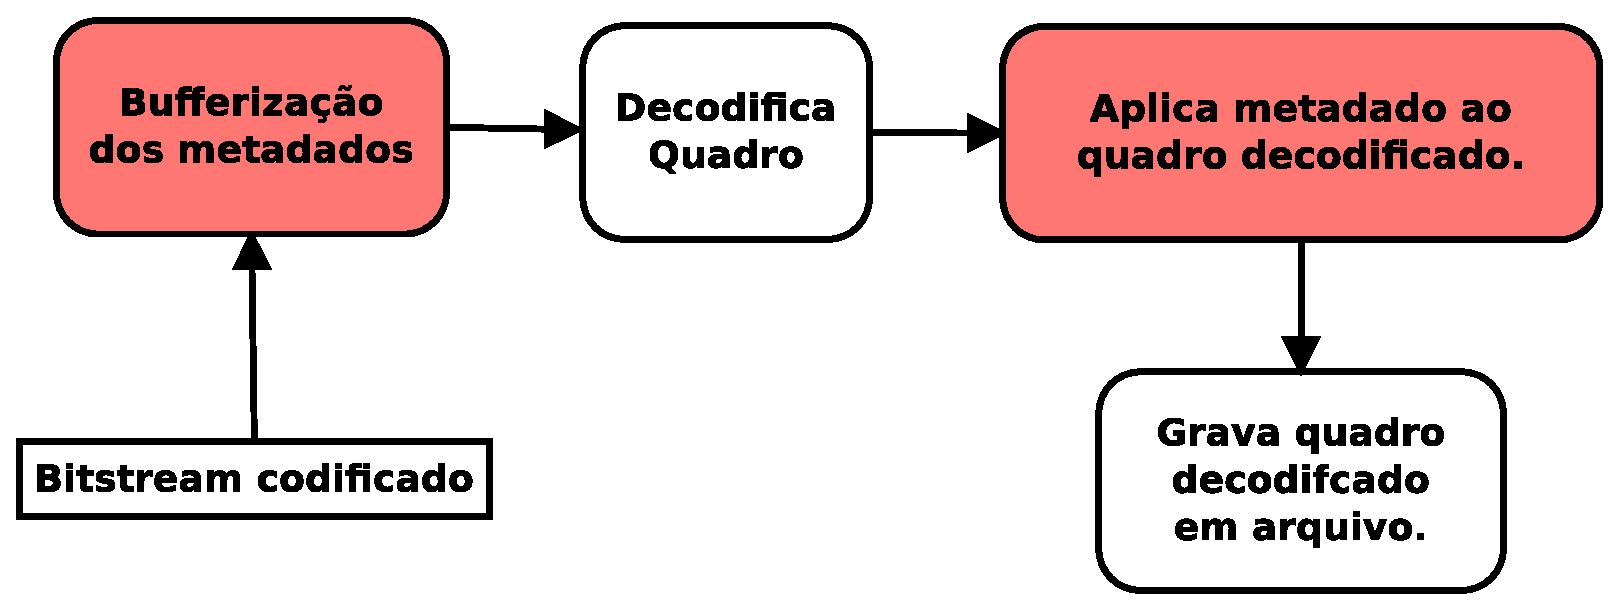
\includegraphics[scale=0.5]{imagens/fig19.eps}
\caption{Visão geral do decodificador H.264 modificado. Os blocos vermelhos representam os processos adicionados ao decodificador.}
\label{fig:h264_moded_decoder}
\end{figure}


\subsection{ Recuperando metadados a partir do bitstream }


Para realizar a recuperação de um metadado previamente inserido no bitstream durante o processo de codificação foi adicionado na estrutura \textit{VideoParameters} (definida em \textit{ldecod/inc/global.h}) do decodificador um novo campo chamado \textit{metadata\_buffer} do tipo \textit{ExtractedMetadataBuffer}. Esse buffer é inicializado na função \textit{main} do decodificador, que se encontra em \textit{ldecod/src/decoder\_test.c}, logo após o decodificador ter sido configurado, mas antes de iniciar o processo de decodificação.

Ao longo do processo de decodificação, sempre que um NALU do tipo SEI é encontrado no bitstream a função \textit{InterpretSEIMessage} é chamada, essa função se encontra em \textit{ldecod/src/sei.c}. Nela existe um \textit{switch case} para os diversos tipos de mensagens SEI possíveis, no \textit{case} \textit{SEI\_USER\_DATA\_UNREGISTERED} foi adicionada detecção se essa mensagem é um \textit{ExtractedMetadata}. Em caso afirmativo, esse metadado será adicionado ao \textit{ExtractedMetadataBuffer}, caso contrário a mensagem é ignorada.


\subsection{ Aplicando o metadado ao quadro }


Depois de receber e bufferizar os metadados foi necessário encontrar um bom lugar para aplicar os metadados ao quadro, de preferência logo antes do quadro ser gravado em arquivo, onde todo o processo de decodificação já teria ocorrido. Foi escolhido o inicio da função \textit{write\_out\_picture}, que se encontra em \textit{ldecod/src/output.c} como melhor local para realizar a aplicação do metadado.

Para auxiliar o processo de aplicação de metadados do tipo \textit{ExtractedObjectBoundingBox} foi adicionado em \textit{ldecod/src/output.c} a função \textit{decoder\_draw\_bounding\_box}, que verifica se o metadado é do tipo \textit{ExtractedObjectBoundingBox}, em caso afirmativo a caixa delimitadora é desenhada no quadro, caso contrário o metadado é ignorado.

No inicio da função \textit{write\_out\_picture} um contador é utilizado para definir o número do quadro (em ordem de apresentação), o número do quadro é utilizado na chamada do método \textit{get} da classe \textit{ExtractedMetadataBuffer}, para verificar a existência de um metadado para aquele quadro. Se um metadado existir para este quadro, será chamada a função \textit{decoder\_draw\_bounding\_box}, que desenhará a caixa delimitadora no quadro.


